\documentclass{article}
\usepackage[space,hyperref,UTF8]{ctex}
\usepackage[backref]{hyperref}%超链接
\usepackage{geometry}
%\usepackage[sort&compress]{gbt7714}%国标参考文献
\geometry{a4paper,left=2.5cm,right=2.5cm,top=2.5cm,bottom=2.5cm}%调整页边距
\usepackage{amsmath}
\usepackage{titlesec}%设置标题字号格
\usepackage{graphicx}
\graphicspath{{图片/}}
\usepackage{booktabs}
\usepackage{amsthm}
\usepackage{lipsum}
\usepackage{float}
\usepackage{fontspec}
\usepackage[dvipsnames,svgnames]{xcolor}

\usepackage[strict]{changepage} % 提供一个 adjustwidth 环境
\usepackage{fancybox}
\usepackage{cases}
\usepackage{tcolorbox}
\usepackage{framed} % 实现方框效果
\usepackage{newtxtext}
\usepackage{xcolor}
\usepackage{color}
\usepackage{caption}
\usepackage{subfigure}
\definecolor{formalshade}{rgb}{0.95,0.95,1} % 文本框颜色
%

% 注意行末需要把空格注释掉,不然画出来的方框会有空白竖线
\newenvironment{formal}{%
	\def\FrameCommand{%
		\hspace{1pt}%
		{\color{DarkBlue}\vrule width 2pt}%
		{\color{formalshade}\vrule width 4pt}%
		\colorbox{formalshade}%
	}%
	\MakeFramed{\advance\hsize-\width\FrameRestore}%
	\noindent\hspace{-4.55pt}% disable indenting first paragraph
	\begin{adjustwidth}{}{7pt}%
		\vspace{2pt}\vspace{2pt}%
	}	{%
		\vspace{2pt}\end{adjustwidth}\endMakeFramed%
}

\title{\songti\zihao{3}毕业设计(论文)开题报告}
\author{王云龙}
\date{\today}

%\newfontfamily\sectionfont{Times New Roman}
\renewcommand\thesection{\chinese{section}}
\renewcommand\thesubsection{\arabic{subsection}}
\renewcommand\thesubsubsection{\arabic{subsection}}	

\titleformat{\section}[block]{\raggedright\large\bfseries}{\thesection\,、}{1em}{}

\titleformat{\subsection}[block]{\raggedright\large\bfseries}{\arabic{section}.\arabic{subsection}}{1em}{}

\titleformat{\subsubsection}[block]{\raggedright\large\bfseries}{\arabic{section}.\arabic{subsection}.\arabic{subsubsection}}{1em}{}

\begin{document}

\maketitle
\fancypage{\fbox}{}
%\tableofcontents
%\bibliographystyle{plain} %参考文献格式
%\bibliography{bibeTex} %参考文件库
\section{课题来源、目的及意义}
回流上古,追溯原始,从三百万年前非洲大陆的石器,到四千年前美索不达米亚的青铜,再到一千四百年前小亚细亚的铁器,人类科技一直以一种小步慢跑的方式发展,直到十八世纪六十年代,英格兰地区蒸汽动力的出现,标志着第一次工业革命的开始,它带领人类从农业文明进入到工业文明,封建经济被资本主义经济取代,完成第一次工业革命的资本主义国家迅速开始全球扩张进行资本积累,十九世纪七十年代,标志着以电气为代表的第二次工业革命的开始,资本主义飞速发展,世界经济格局、资本主义世界市场形成,促进了工人运动和社会主义运动,第二次世界大战后,世界出现新格局,以美国为首的北约和以苏联为首的华约之间的冷战,诞生了超乎人类想象力的科技,如通用电器公司的Hardiman-动力装甲,SR-71黑鸟式侦察机,XB-70女武神式战略轰炸机,阿波罗计划,地效飞行器,核潜艇等。

纵观人类科技发展历史,从最初的小步慢跑到井喷式发展,每一个扩展人类想象力科技的背后都离不开工业机器的自动化生产,而当今世界正处于第四次工业革命的浪潮中,以人工智能,大数据、机器人为代表的新技术正推动着工业生产进行新一轮的变革,工业自动化,信息化、智能化逐渐成为未来制造业的发展趋势,传统制造业对于产业转型的需求日益迫切,在此背景下,国务院于2015年5月提出《中国制造2025》十年行动纲领,目的就是为了加快推动新一代信息技术与传统制造业融合发展,将智能制造作为主攻方向,着力发展智能装备和智能产品,推进生产过程智能化,机器人凭借着强大的通用性,逐渐成为产业转型中的核心设备,而新兴的人工智能和大数据则赋予机器人更加智能化,据中研产业研究院发布的《2019-2025年中国机器人行业全景调研与发展战略研究咨询报告》显示,自2018年以来,随着中国机器人产业的迅速发展,产品结构延续近几年发展态势,附加值高的国产多关节机器人销量不断提升,产品结构呈现优化态势。随着中国机器人相关技术特别是附加值高产品技术的不断提升,多关节机器人产品性能将进一步得到完善。同时企业自身不断积极优化产品结构、提高制造水平,国产多关节机器人销量将进一步提升。

在工业生产中,机器人通常代替人工进行复杂而危险的操作,比如利用机器人进行搬运物体,切割、焊接金属,装配零件等,常用的示教机器人需要技术人员基于目标位置,综合考虑路径等因素提前对机器人进行编程,而且所能进行的操作有限,动作简单,一旦环境改变,将要对其重新编程,这样不仅增加人力成本,而且定位精度也会受到一定的影响。

随着机器视觉的发展,人们将机器人技术与机器视觉结合起来,通过机器视觉系统对目标物体进行识别与定位,然后将位置信息发送给机器人,从而自主到达目标位置实现相应操作,摆脱了传统示教机器人提前编程的繁琐方法,而且机器视觉定位精度高,处理速度快,能对物体进行实时检测,具有很强的适应环境的能力,两项技术的结合使机器人变得更加智能化,应用更加广泛,大大提高了生产效率,降低了生产成本,工业生产变得更加自动化,智能化。

机器人在抓取物体过程中,涉及不同的坐标系之间的变换,因此视觉标定则是实现机器人定位抓取的重要前提,通过相机标定我们可以得到三维世界的物体与像素点的对应关系,这样我们就可以通过视觉系统拍摄的图像来获取物体在三维世界坐标系下的坐标,此时的坐标是相对于相机坐标系的,我们再通过手眼标定来将其坐标转换到机器人基座坐标系下,于是我们就可以根据机器人逆运动学求解出D-H矩阵,从而控制各个关节的旋转角度,移动到相应位置实现定位抓取操作。









\section{国内外研究或生产现状}
机器视觉作为实现机器人抓取的重要前提,其中视觉标定就显得尤为重要,是获取物体三维信息的重要途径,本文主要研究相机的视觉标定方法设计,根据求解方法及参考物的不同,相机标定主要分为以下三种类型:
\begin{itemize}
	\item 传统标定方法
	\item 相机自标定
	\item 主动视觉标定法
\end{itemize}
\subsection{国内}

\begin{description}
	\item[传统标定方法] 国内对相机标定研究起步较晚,最具代表性的是在1998年张正友出的一种以平面棋盘格为标定物的标定方法,传统标定法的标定板是需要三维的,需要非常精确,这很难制作,而张正友教授提出的方法介于传统标定法和自标定法之间,克服了传统标定法需要的高精度标定物的缺点,而仅需使用一个打印出来的棋盘格就可以。同时也相对于自标定而言,提高了精度,便于操作。韩龙提出利用标定板上各角点间的约束关系提高张氏标定法的标定精度。2015年文涛等提出利用交叉网格作为参照物进行标定,在复杂光照条件下可以准确获取信息。2016年徐中宇等针对传统方法易出现局部最优解的问题,将遗传算法应用于相机参数优化中,大大提高了标定精度。2017 年田楠楠提出五点标定法,简化了模板的复杂度,从结果上看精度略高于传统算法。王道累等人在2020年提出将天牛须搜索算法应用到标定参数优化中,在实验中表明该方法能有效提高参数收敛速度
	
	\item[相机自标定] 我国的孟晓桥在2000年首次提出使用圆环作为参照物,将圆环在透视投影中的重要特性引入到自标定理论中,极大的促进了相机标定技术的发展。在2012年陈天飞等提出了不使用参照物就可以实现相机自标定的方法,但精度较低,算法鲁棒性差。徐建平等在2015年将粒子群算法与自标定技术相结合,提高了自标定的精度和收敛速度。	
	
	\item[主动视觉标定法] 主动视觉法是根据相机的运动轨迹来求解相关参数。雷成等从数学角度进一步推导出空间点的重建以及利用极点信息求解外参矩阵的条件。
\end{description}



\subsection{国外}
\begin{description}
	\item[传统标定方法] 在1971年Abdel-Aziz根据透视原理提出了直接线性变换法,但由于缺乏对参数之间的约束和镜头畸变的考虑,故而标定精度不高。随着标定技术的发展,在1987年Tsai提出的两步法加入了对径向畸变的考虑。而后J.Weng在两步法的基础上增加了对切向
	畸变的考虑,可适用于失真严重的场合下。
	
	\item[相机自标定] Hartley和Faugeras在1992年首次提出相机自标定方法,利用射影几何和极线约束对相机进行标定。自标定法仅通过匹配目标图像上相互对应的特征点,按照约束关系建立多元方程就可得到标定参数,但其精度不如传统方法高。同年Faugeras提出在内参固定的情况下,可以通过求解图像间的Kruppa方程,从而求解参数。
		
	\item[主动视觉标定法] 马颂德所提出利用三正交运动进行标定就是一种标准的主动视觉法。主动视觉法不同于前两种方法,需要明确相机
	的运动轨迹,且对实验设备的要求高,需要特定装置(如编码器、位移台等外部设备)控制相机做特殊运动。
	
\end{description}
\section{课题研究内容及实施方案}
\subsection{研究内容}
\subsubsection{相机标定的目的与原理}
相机标定是一种转换关系,将三维世界坐标系中的物体与拍摄的二维图像坐标系中的像素点之间的对应关系抽象为一种数学描述,这种数学描述可以用矩阵来表示,通过相机标定,可以获得具有实际意义的数据:
	\begin{itemize}
		\item 外参矩阵$M_2$:三维世界的物体如何通过旋转和平移到达相机坐标系
		\item 内参矩阵$M_1$:相机内部的几何和光学特性
		\item 畸变系数:小孔成像模型没有考虑相机镜头对成像的影响,导致像素点没有落在理论位置上,产生了偏移和变形
		\item 结构参数:左右相机的位置关系	
	\end{itemize}

相机标定根据特征点提取难度可分为:
	\begin{itemize}
		\item 相机自标定:通过图像处理提取特征点,主要包含以下步骤:
		\begin{itemize}
			\item 图像灰度化
			\item 图像滤波
			\item 图像二值化
			\item Canny边缘检测
			\item Harris亚像素级角点检测
		\end{itemize}
		\item 标定板标定:特征点为黑白棋盘格角点,易求
	\end{itemize}
相机标定按照相机是否静止,可分为:
\begin{itemize}
	\item 静态相机标定:标定板运动,相机静止
	\item 动态相机标定:标定板静止,相机运动
\end{itemize}

\subsubsection{相机模型}
小孔成像模型原理简单,没有镜头,只有一个小孔(类似相机光圈),三维世界的物体反射太阳光线通过小孔投影到成像表面,如图\ref{小孔成像模型}所示:
\begin{figure}[H]
\begin{center}
	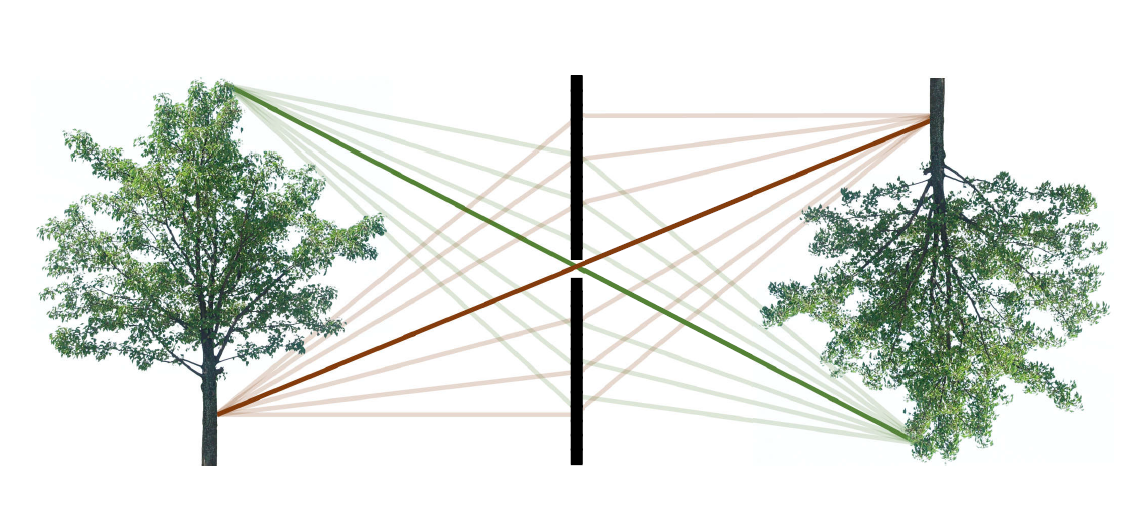
\includegraphics[scale=0.3]{小孔成像模型1}
	\caption{小孔成像模型示意图}
	\label{小孔成像模型}
\end{center}
\end{figure}

小孔成像模型得到的是倒立的虚像,其成像原理及简化示意图如图\ref{小孔成像原理及简化示意图}所示,其数学描述如式(\ref{小孔成像模型-公式描述负号})所示:

\begin{figure}[H]
	\centering  %居中
	\subfigure[实际物体投影]{   %第一张子图
		\begin{minipage}{7cm}
			\centering    %子图居中
			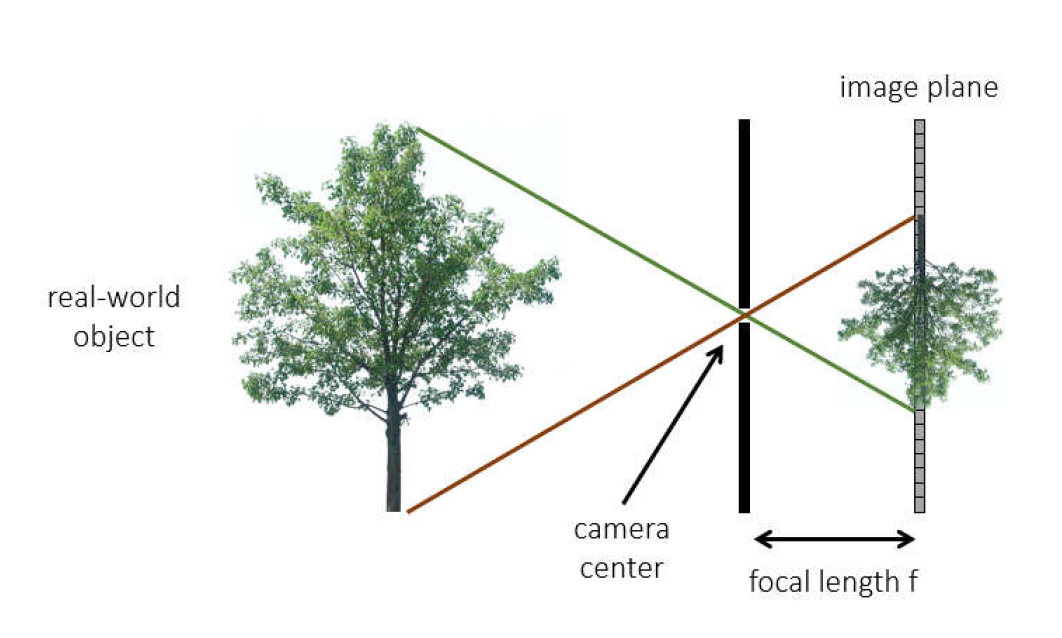
\includegraphics[scale=0.22]{小孔成像模型2}  %以pic.jpg的0.5倍大小输出
		\end{minipage}
	}
	\subfigure[简化示意图]{ %第二张子图
		\begin{minipage}{7cm}
			\centering    %子图居中
			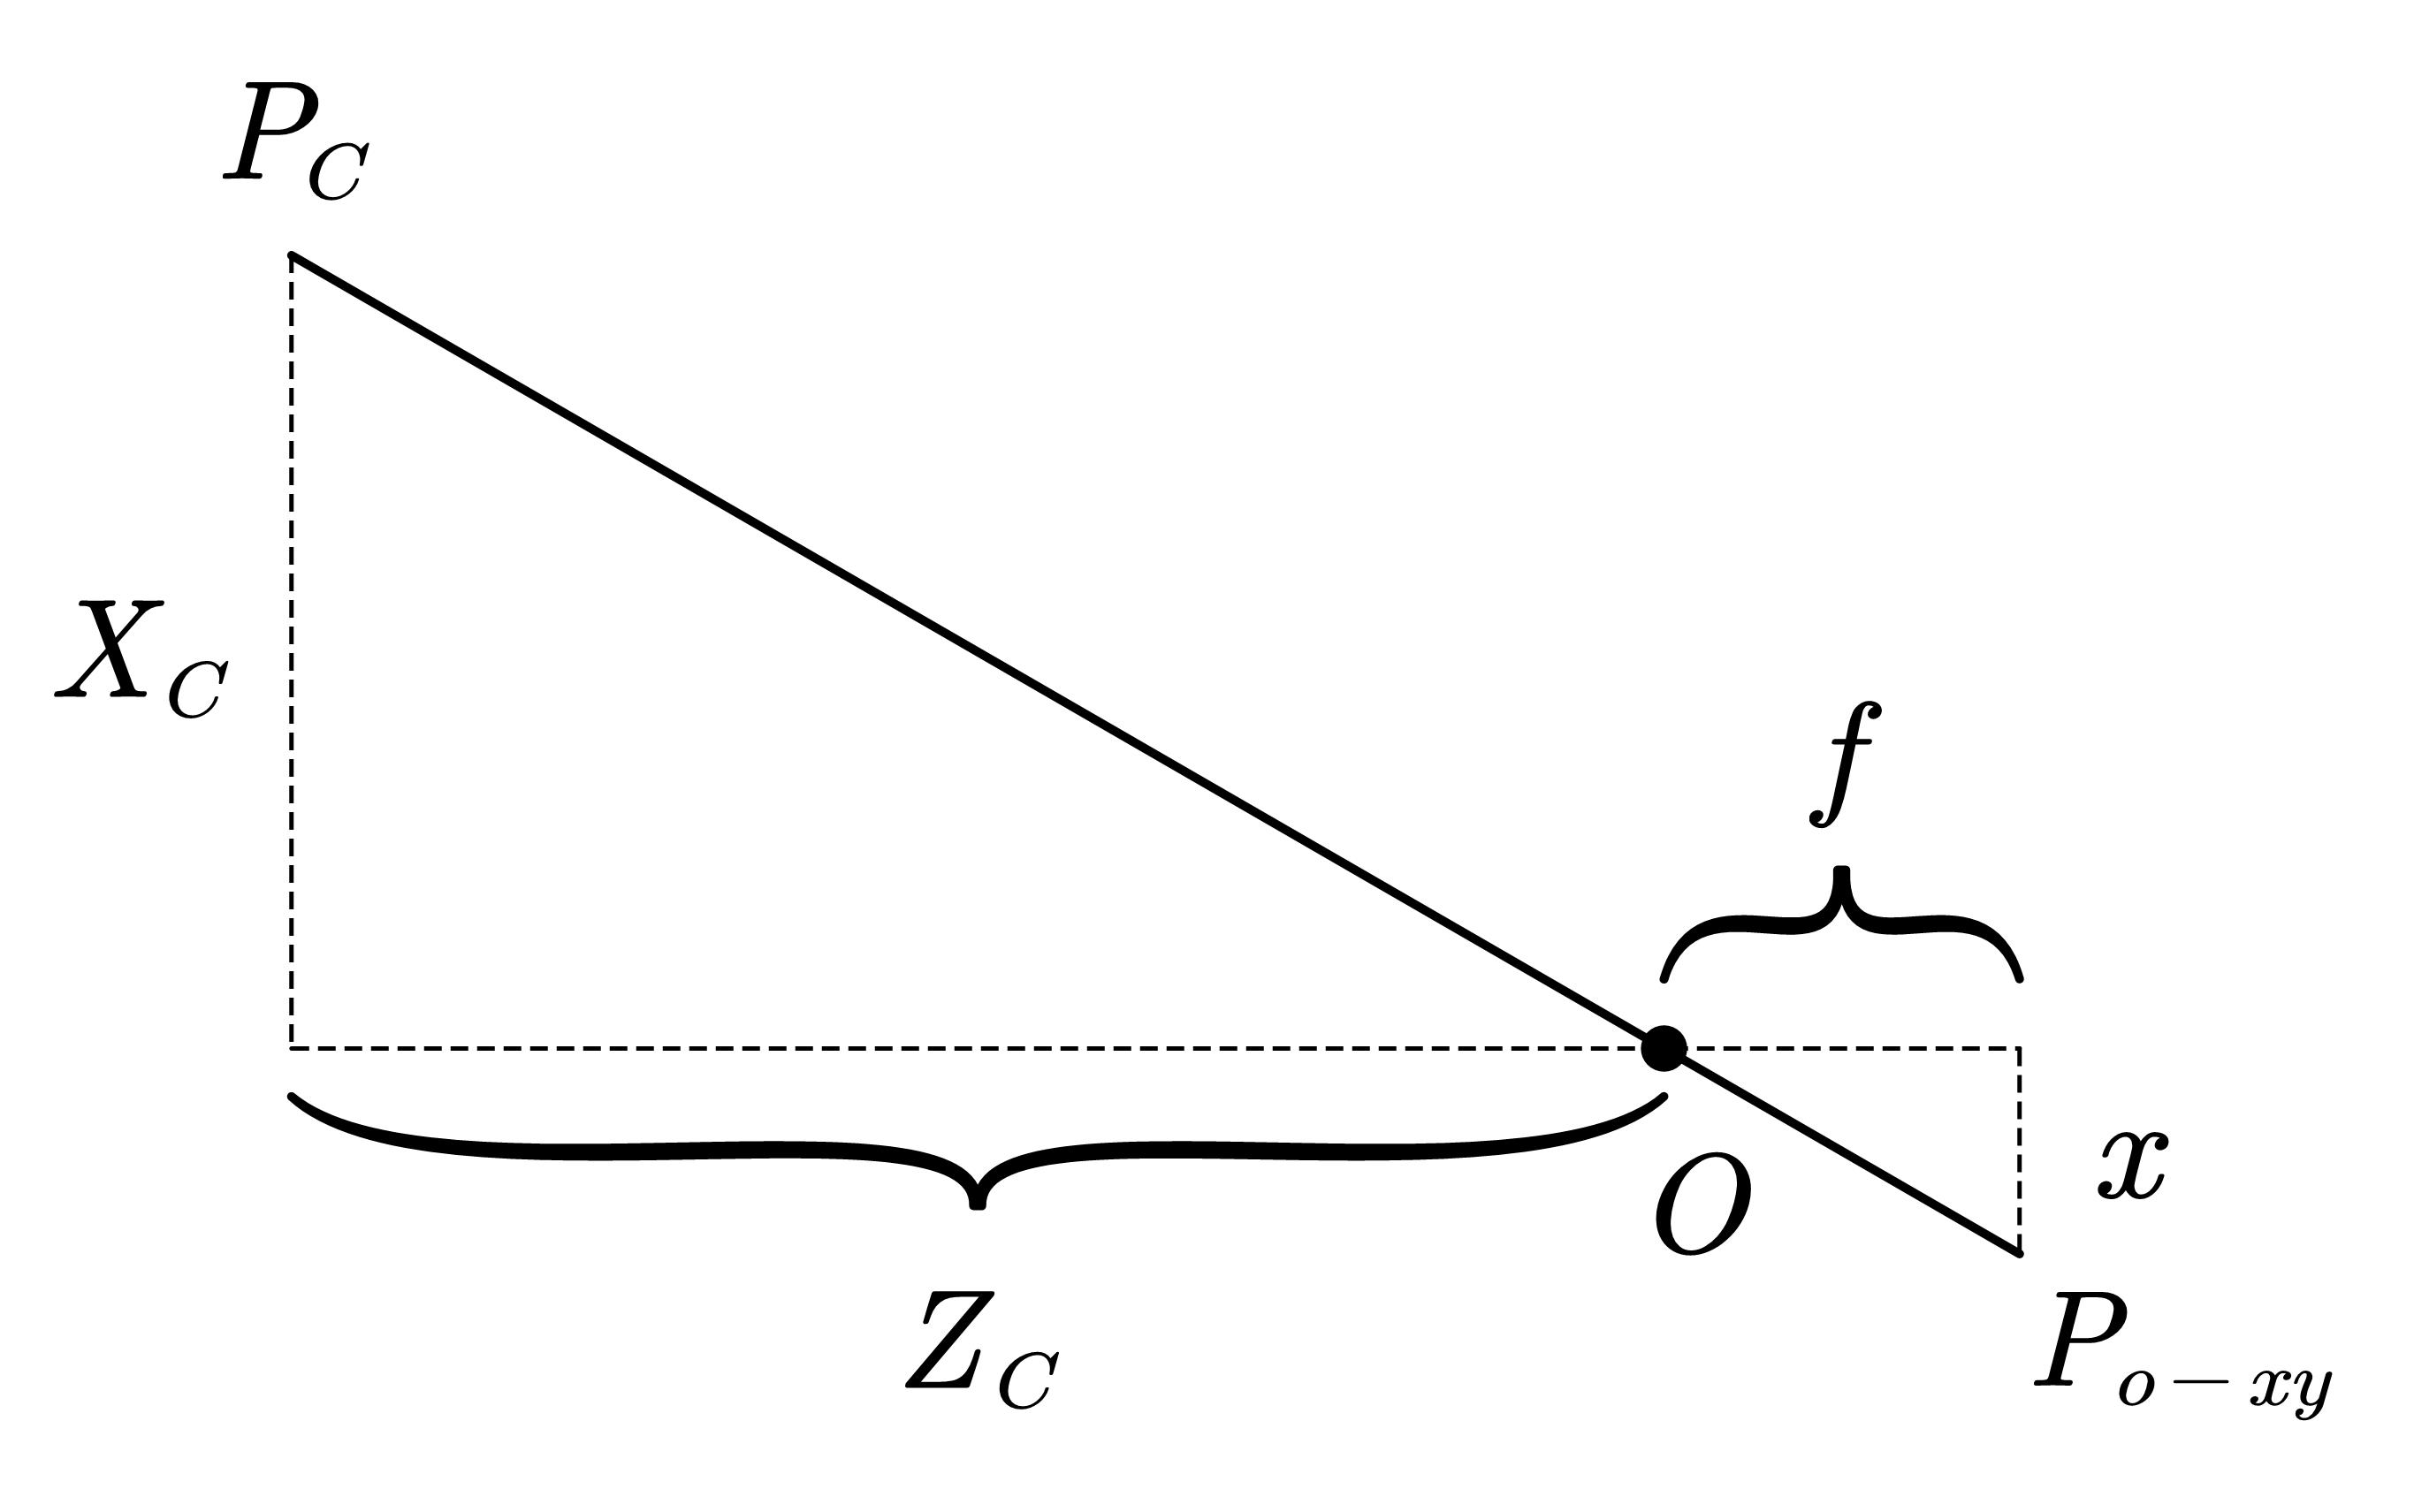
\includegraphics[scale=0.55]{小孔成像模型原理1}
		\end{minipage}
	}
	\caption{小孔成像原理及简化示意图}    %大图名称
	\label{小孔成像原理及简化示意图}    %图片引用标记
\end{figure}
\begin{gather}
	\left\{ \begin{array}{c}
		x=-f\cdot \frac{X_c}{Z_c}\\
		\\
		y=-f\cdot \frac{Y_c}{Z_c}\\
	\end{array} \right. 	\label{小孔成像模型-公式描述负号}
\end{gather}

可以看到,式(\ref{小孔成像模型-公式描述负号})含有符号,为了后面的计算方便,我们将成像投影到前面以消除负号,改进后的成像原理及简化示意图如图\ref{小孔成像原理及简化示意图-改进}所示,其数学描述如式(\ref{小孔成像模型-公式描述负号-改进})所示:
\begin{figure}[H]
	\centering  %居中
	\subfigure[实际物体投影]{   %第一张子图
		\begin{minipage}{7cm}
			\centering    %子图居中
		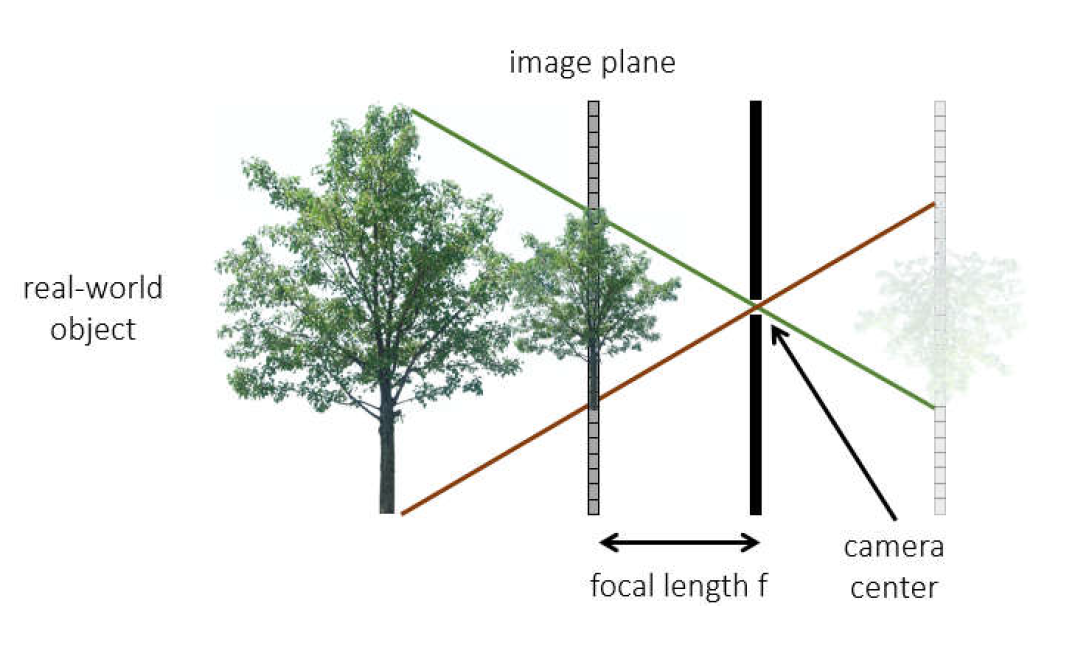
\includegraphics[scale=0.22]{小孔成像模型3}
		\end{minipage}
	}
	\subfigure[简化示意图]{ %第二张子图
		\begin{minipage}{7cm}
			\centering    %子图居中
			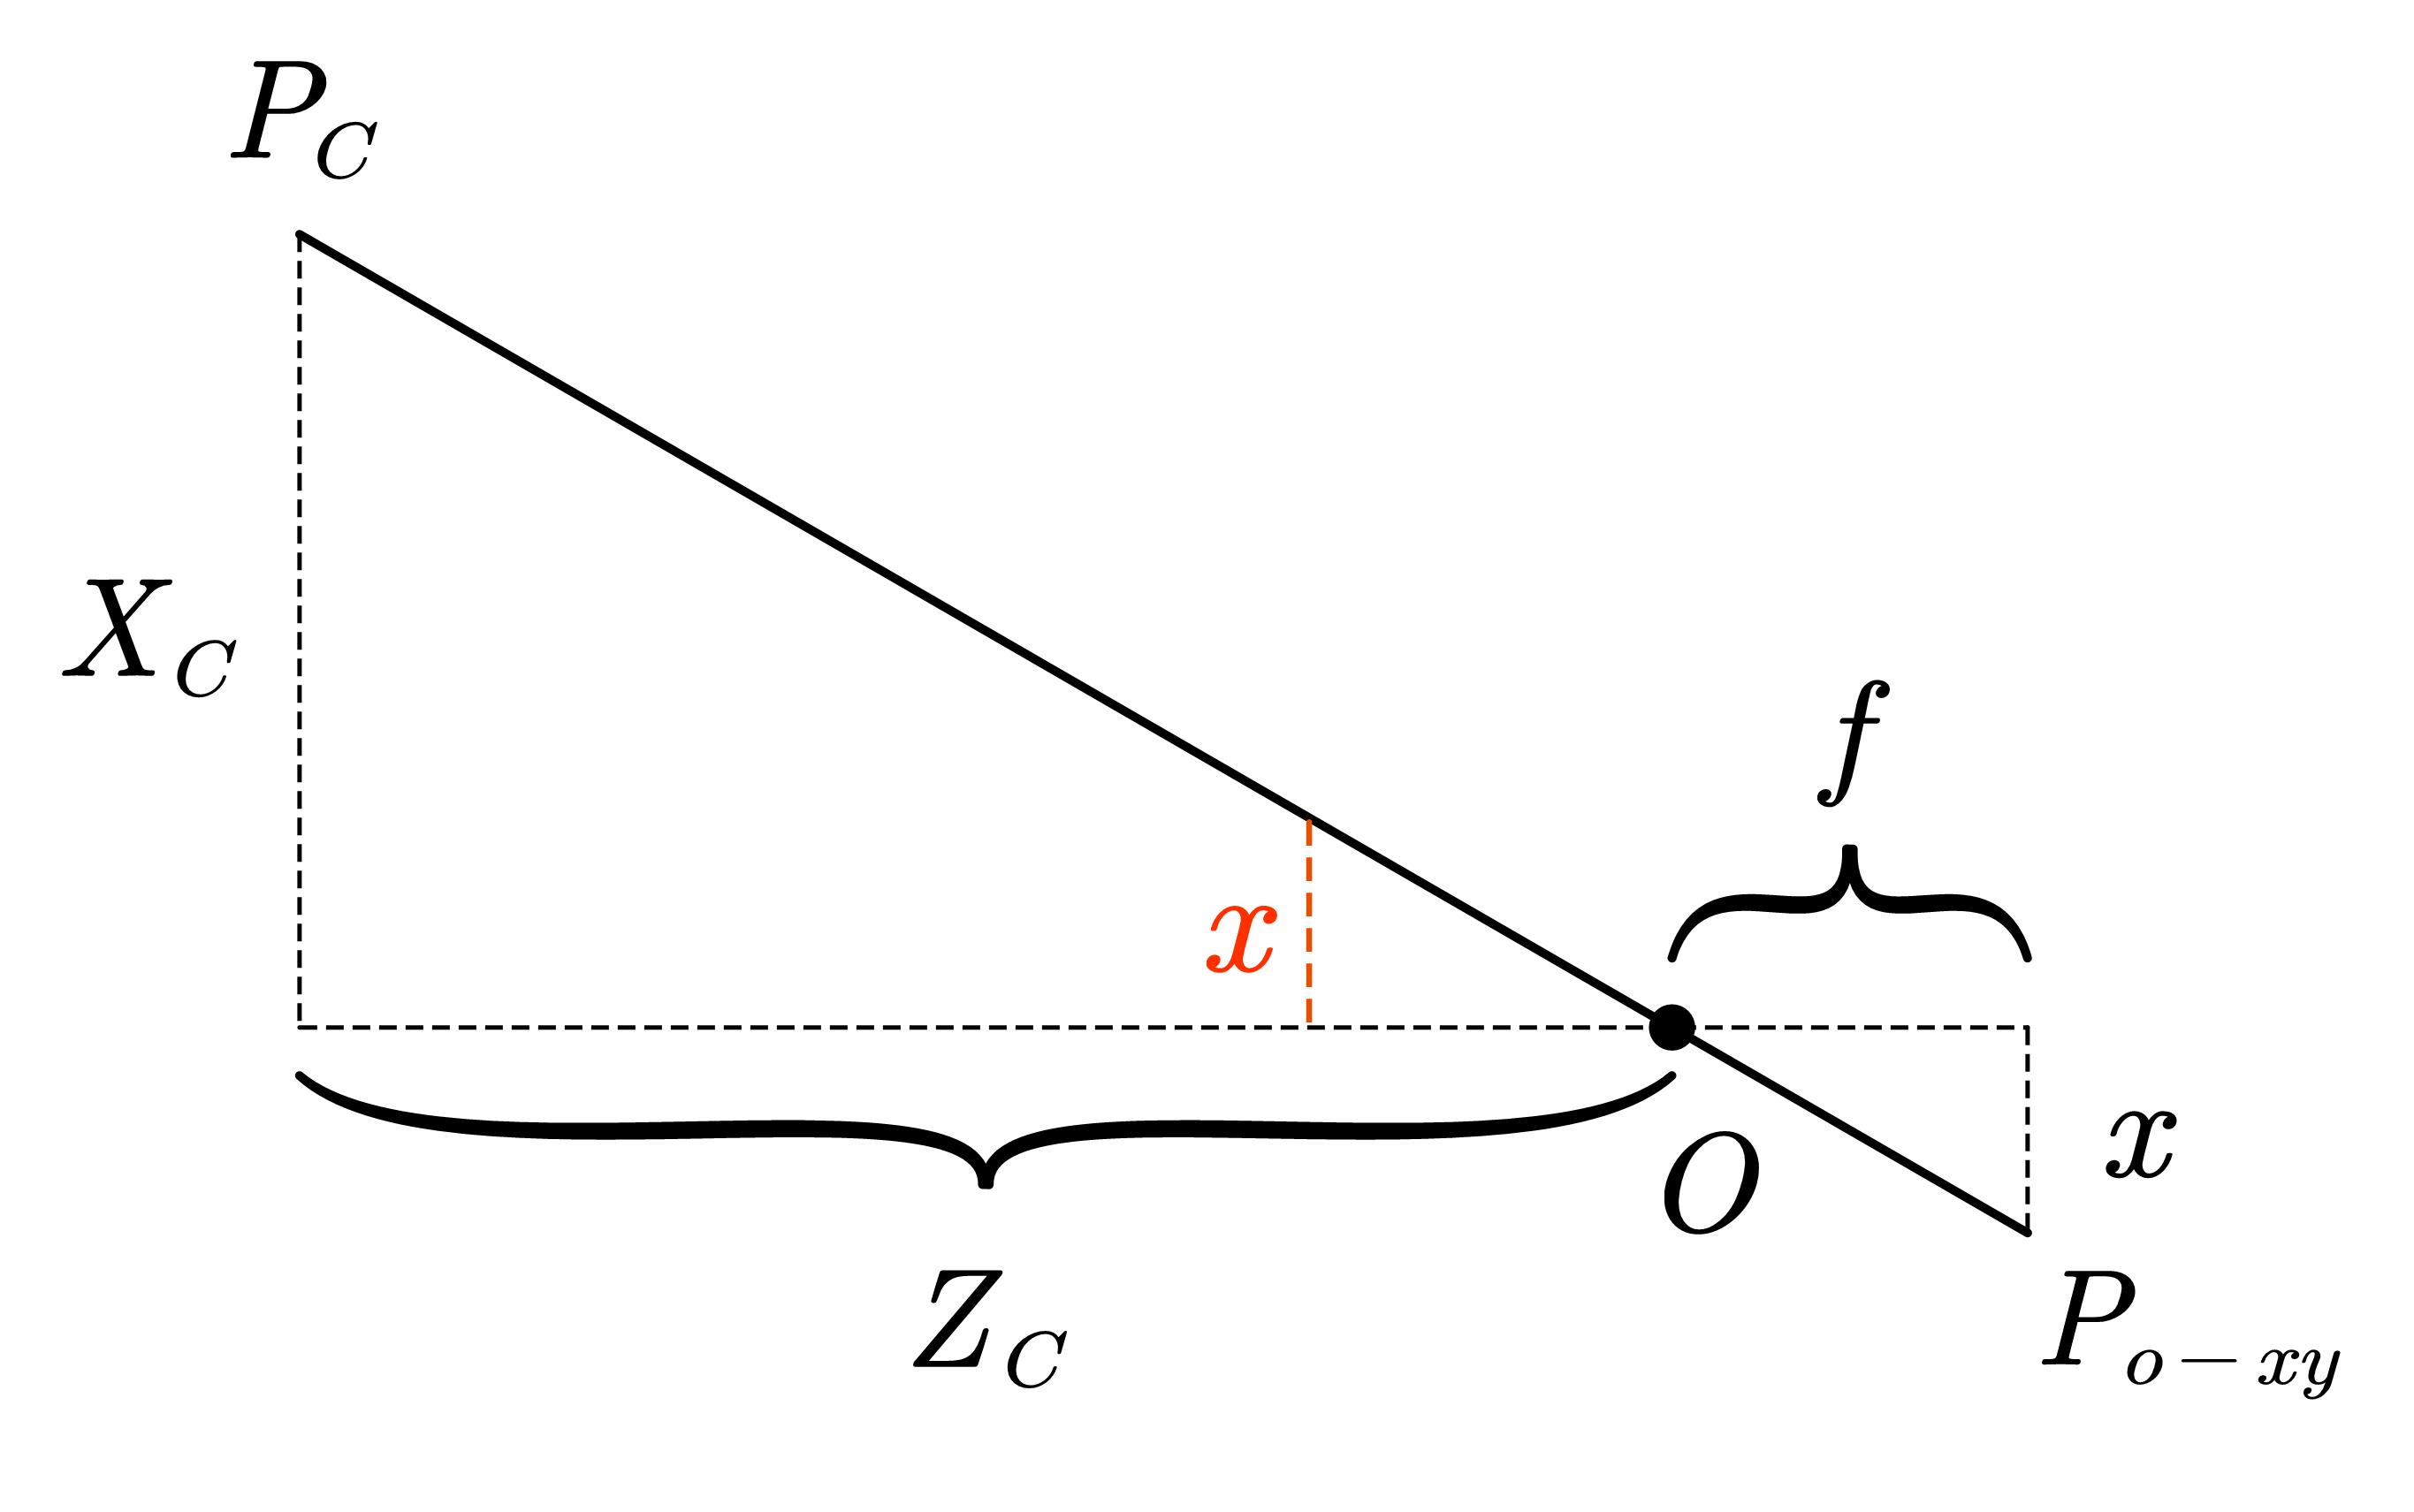
\includegraphics[scale=0.55]{小孔成像模型原理2}
		\end{minipage}
	}
	\caption{改进的小孔成像原理及简化示意图}    %大图名称
	\label{小孔成像原理及简化示意图-改进}    %图片引用标记
\end{figure}
	\begin{gather}
	\left\{ \begin{array}{c}
		x=f\cdot \frac{X_c}{Z_c}\\
		\\
		y=f\cdot \frac{Y_c}{Z_c}\\
	\end{array} \right. 	\label{小孔成像模型-公式描述负号-改进}
\end{gather}
\subsubsection{相机畸变}
为了获得好的成像效果,我们在相机的前方加了透镜,透镜的加入对成像过程中光线的传播会产生新的影响:
\begin{itemize}
	\item 透镜自身的形状对光线传播的影响
	\item 透镜和成像平面不能完全平行,物体投影的位置发生变化
\end{itemize}

于是我们将畸变分为径向和切向畸变:
\begin{itemize}
	\item 径向畸变:透镜形状引起,分为桶型和枕型畸变,如图\ref{径向畸变}所示
	\begin{itemize}
		\item 桶型畸变:离光轴距离越远,图像放大率越小
		\item 枕型畸变:离光轴距离越远,图像放大率越小
		\begin{figure}[H]
		\begin{center}
			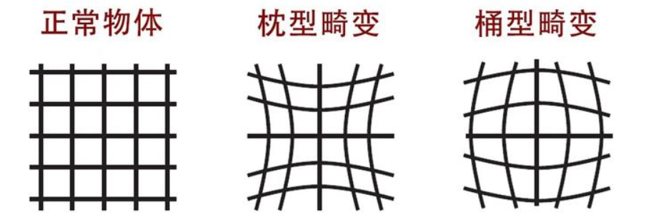
\includegraphics[scale = 0.35]{畸变失真}
			\caption{径向畸变}
			\label{径向畸变}
		\end{center}
		\end{figure}
	\end{itemize}

径向畸变可以用式(\ref{径向畸变-公式描述1})及(\ref{径向畸变-公式描述2})来描述:
\begin{gather}
	x_{corrected}=x\left( 1+k_1r^2+k_2r^4+k_3r^6 \right) \label{径向畸变-公式描述1}
	\\
	y_{corrected}=y\left( 1+k_1r^2+k_2r^4+k_3r^6 \right) \label{径向畸变-公式描述2}	
\end{gather}

其中:
	\begin{itemize}
	\item $(x,y)$是没有畸变的像素点
	\item $(x_{corrected},y_{corrected})$是畸变后的位置
	\item 参数:${\color{red} k_1},{\color{red} k_2},{\color{blue} k_3}$\footnote{一般使用前两项,鱼眼相机使用第三项}
\end{itemize}

	\item 切向畸变:透镜与成像平面不平行,如图\ref{切向畸变}所示:
	\begin{figure}[H]
	\begin{center}
			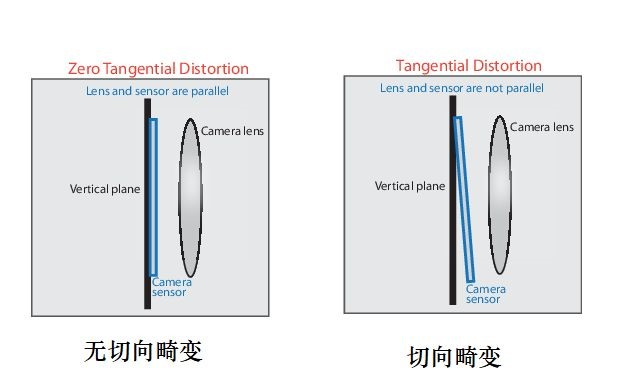
\includegraphics[scale=0.35]{切向畸变.jpg}
			\caption{切向畸变}
			\label{切向畸变}
	\end{center}
	\end{figure}
	
切向畸变可以用式(\ref{切向畸变公式1})及(\ref{切向畸变公式2})来描述:
	\begin{gather}
		x_{corrected}=x+2p_1xy+p_2\left( r^2+2x^2 \right)  \label{切向畸变公式1}
	\\
		y_{corrected}=y+p_1\left( r^2+2y^2 \right) +2p_2xy \label{切向畸变公式2}
	\end{gather}
\end{itemize}

我们将以上两种畸变进行合并,得到如式(\ref{畸变合并1})及(\ref{畸变合并2})的表达式:
	\begin{gather}
	x_{corrected}=x\left( 1+k_1r^2+k_2r^4+k_3r^6 \right) +{\color[RGB]{128, 0, 255} \left[ 2p_1xy+p_2\left( r^2+2x^2 \right) \right] } \label{畸变合并1}
	\\
	y_{corrected}=y\left( 1+k_1r^2+k_2r^4+k_3r^6 \right) +{\color[RGB]{128, 0, 255} \left[ 2p_2xy+p_1\left( r^2+2y^2 \right) \right] }	\label{畸变合并2}
\end{gather}







\subsubsection{数理基础:矩阵、坐标系、齐次坐标}
相机标定是用矩阵来描述的,而矩阵之间的变换涉及不同的坐标系,坐标系涉及以下四种:
	\begin{itemize}
		\item 世界坐标系(3D):描述相机在三维世界的坐标,坐标系用$O_{W} -X_{W} Y_{W} Z_{W} $表示,单位$m$,双目视觉中一般将世界坐标系原点定在左相机或者右相机或者二者$X$轴方向的中点
		\item 相机坐标系(3D):以相机光学中心为原点,$Z$轴与相机光轴重合,坐标系用$O_{C} -X_{C} Y_{C} Z_{C} $表示,单位$m$
		\item 图像坐标系(2D):二维图像的中心点为原点,坐标系用$o-xy$表示,单位$mm$
		\item 像素坐标系(2D):图像的基本单位是像素($pixel$),图像的像素值以矩阵形式保存,坐标原点在图像左上角,坐标系用$o-uv $表示,单位为像素($pixel$)
	\end{itemize}

矩阵主要有以下几种:
\begin{itemize}
		\item 内参矩阵$M_1$:相机坐标(3D)如何变换到像素坐标(2D)
		\item 外参矩阵$M_2$:世界坐标(3D)如何变换到相机坐标(3D)
	\begin{itemize}
		\item 平移矩阵:$T$
		\item 旋转矩阵:$R=R_X\cdot R_Y\cdot R_Z$
		\begin{itemize}
			\item 绕Z轴旋转:$R_Z$
			\item 绕X轴旋转:$R_X$
			\item 绕Y轴旋转:$R_Y$
		\end{itemize}
	\end{itemize}
	\item 单应性矩阵$H$:世界坐标系(3D)与像素坐标系(2D)之间的映射关系
	\end{itemize}

其中对于旋转矩阵来说,绕Z轴旋转有以下描述:
\begin{gather}
	R_Z\left( \theta \right) =\left[ \begin{matrix}
	\cos \theta&		-\sin \theta&		0\\
	\sin \theta&		\cos \theta&		0\\
	0&		0&		1\\
	\end{matrix} \right] 	
\end{gather}	

\begin{figure}[H]
	\begin{center}
		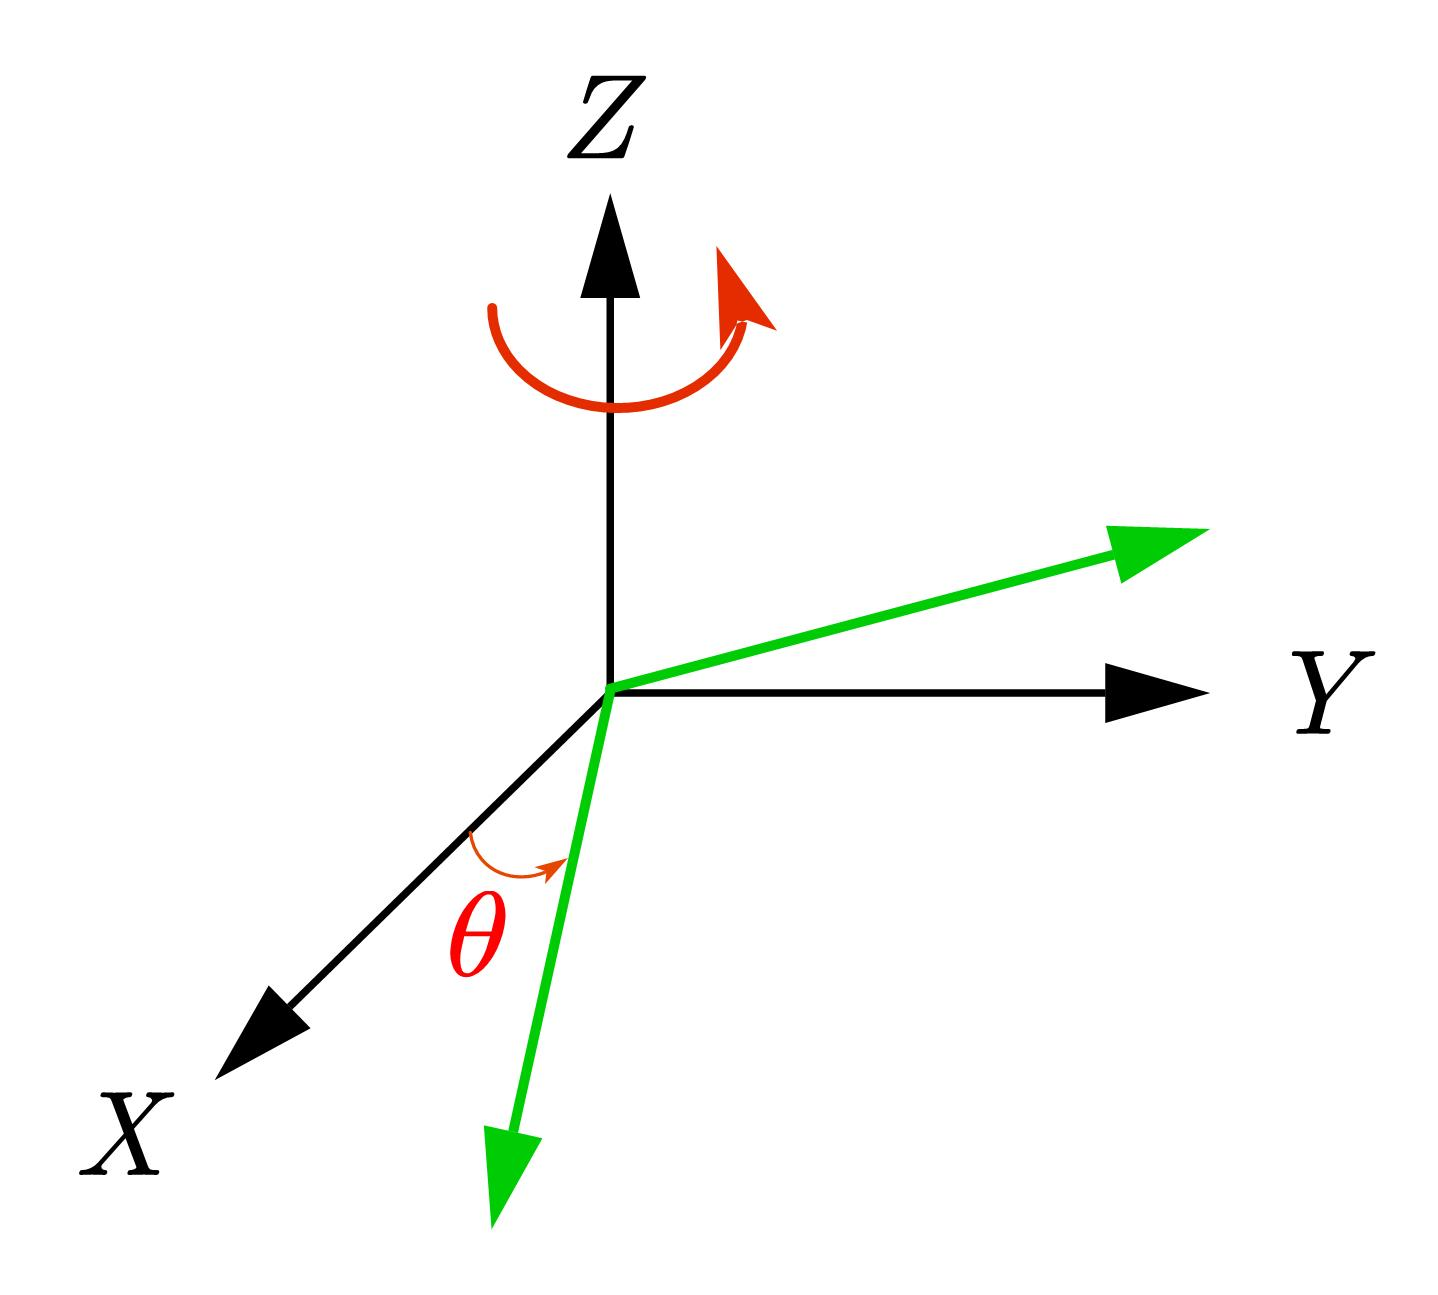
\includegraphics{旋转矩阵Z}
		\caption{绕Z轴旋转}
		\label{绕Z轴旋转}
	\end{center}
\end{figure}

绕X轴旋转有以下描述:
\begin{gather}
	R_X\left( \theta \right) =\left[ \begin{matrix}
		1&		0&		0\\
		0&		\cos \theta&		-\sin \theta\\
		0&		\sin \theta&		\cos \theta\\
	\end{matrix} \right] 	
\end{gather}

\begin{figure}[H]
	\begin{center}
		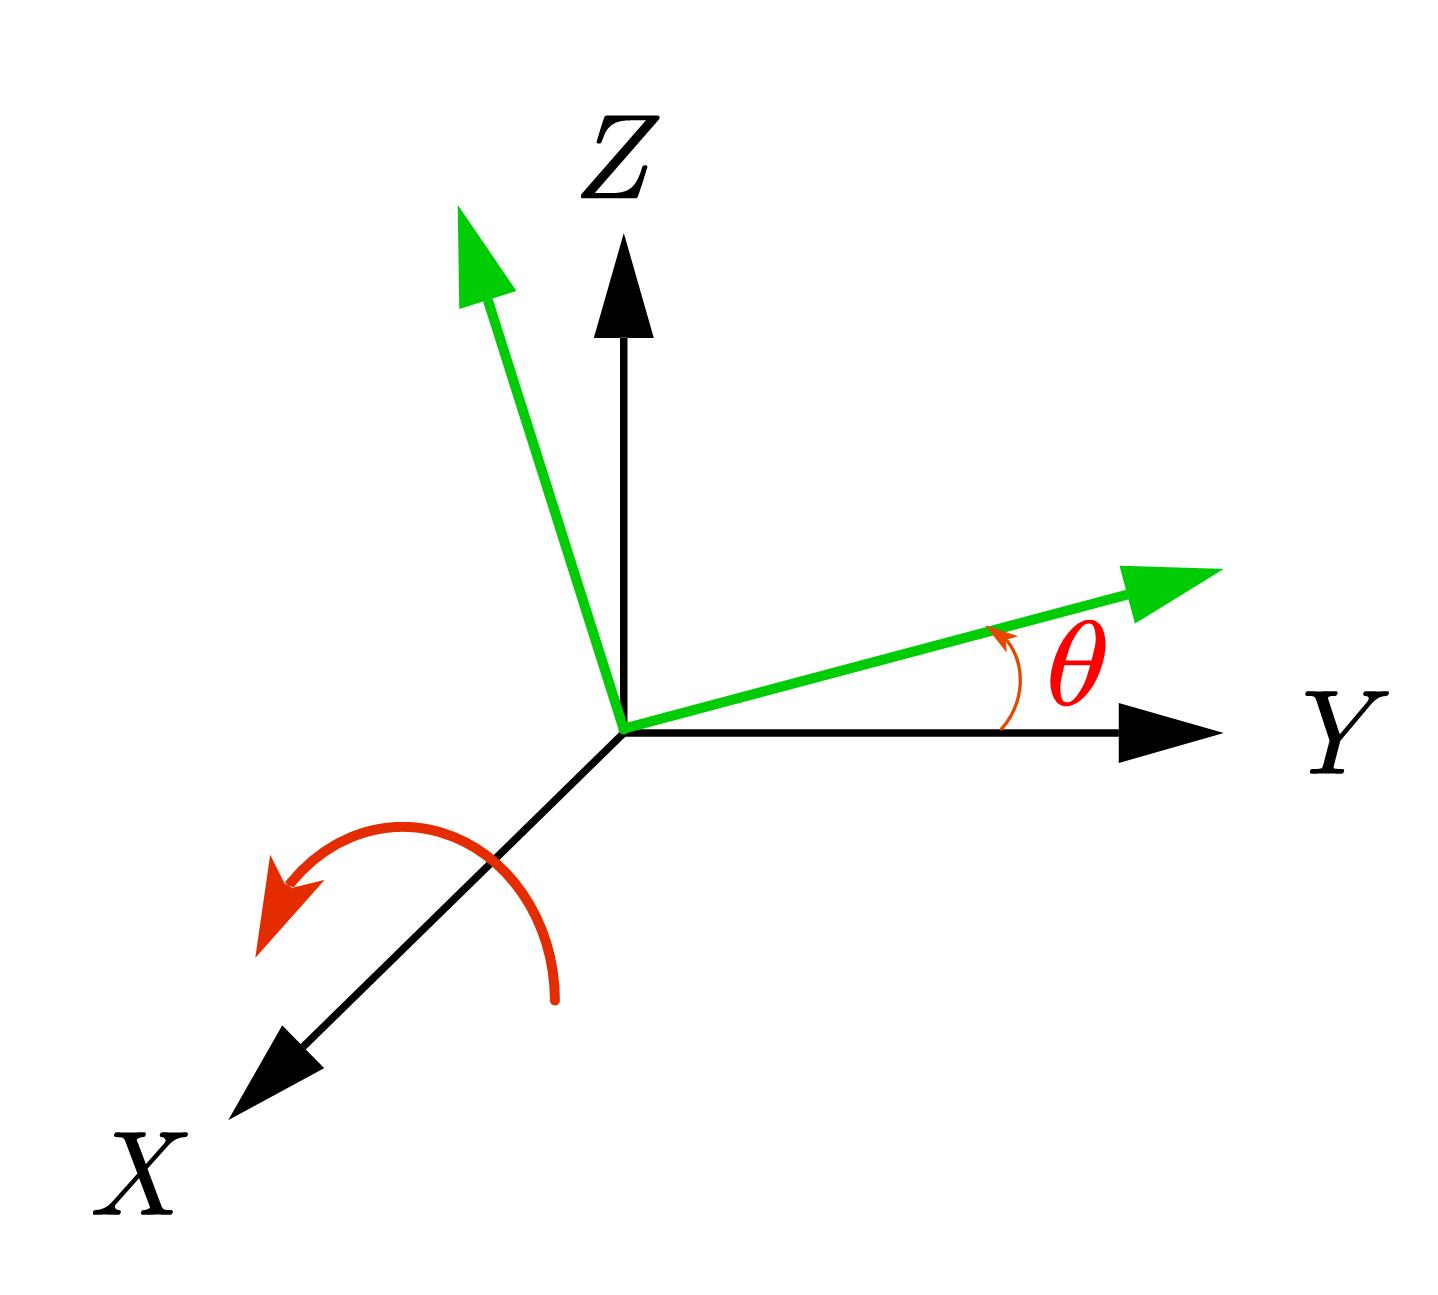
\includegraphics{旋转矩阵X}
		\caption{绕X轴旋转}
		\label{绕X轴旋转}
	\end{center}
\end{figure}

绕Y轴旋转有以下描述:
\begin{gather}
	R_Y\left( \theta \right) =\left[ \begin{matrix}
		\cos \theta&		0&		\sin \theta\\
		0&		1&		0\\
		-\sin \theta&		0&		\cos \theta\\
	\end{matrix} \right] 		
\end{gather}

\begin{figure}[H]
	\begin{center}
		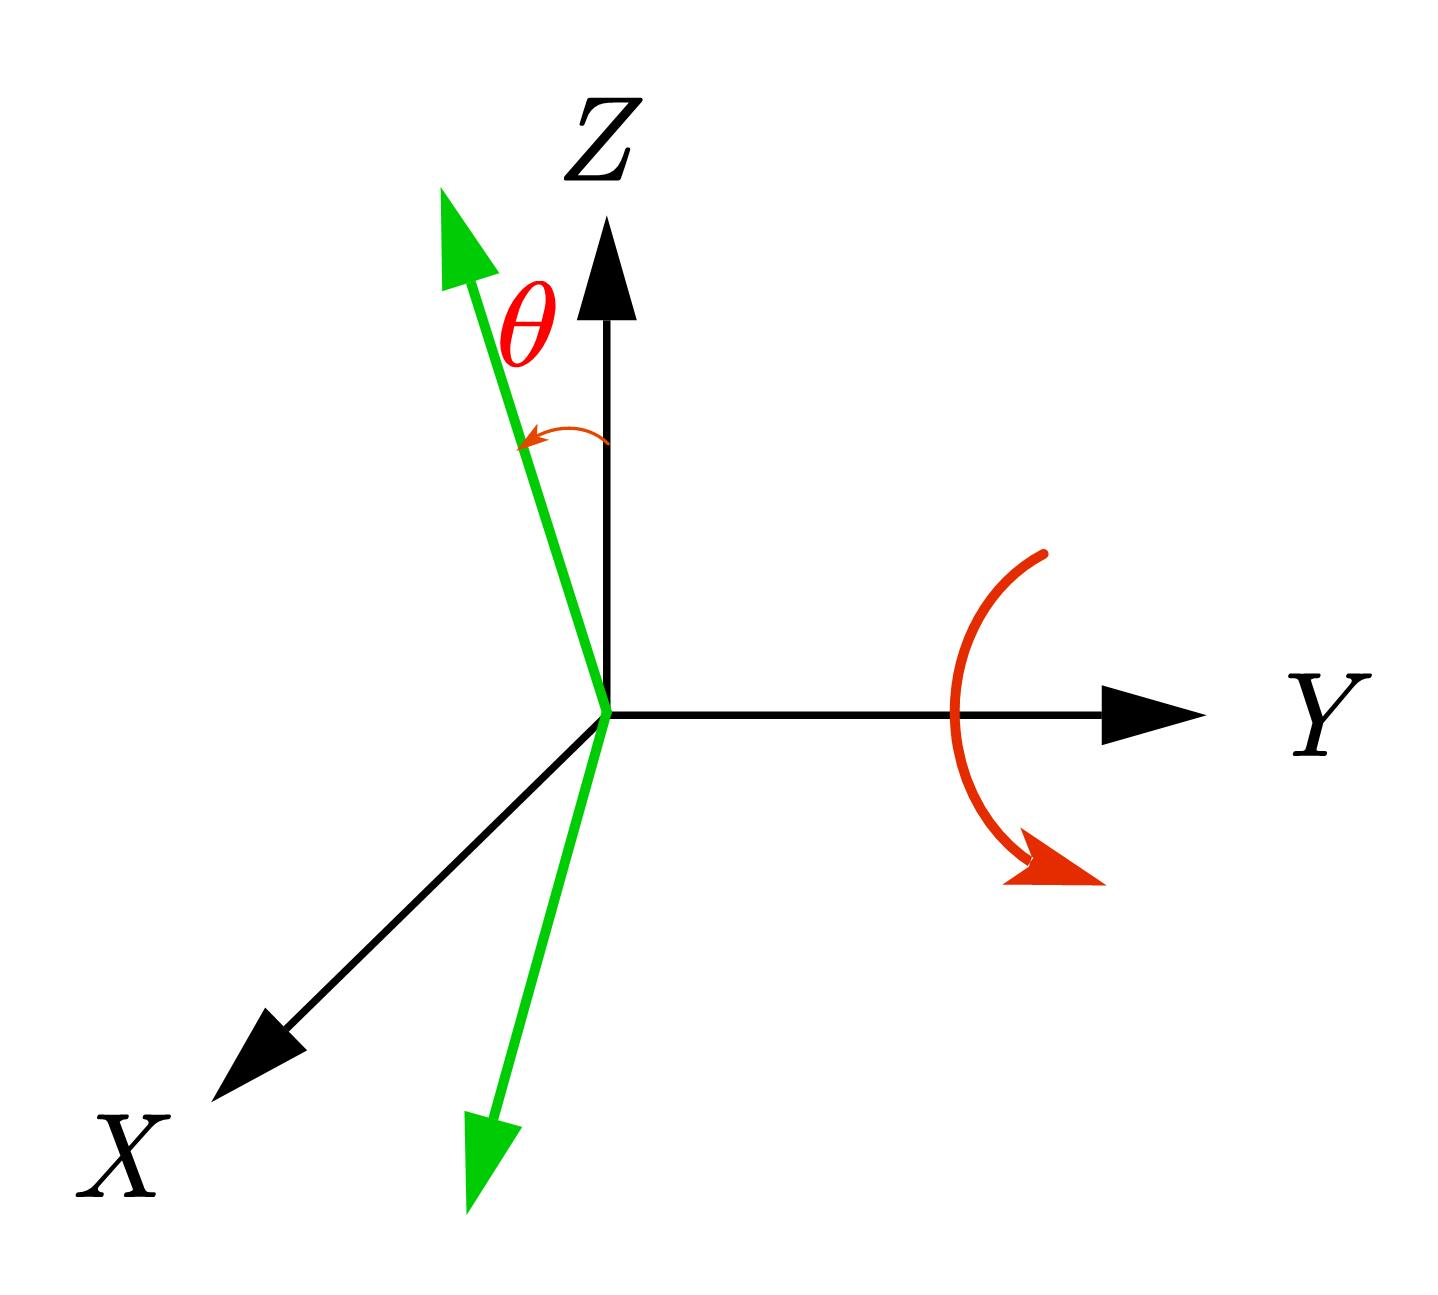
\includegraphics{旋转矩阵Y}
		\caption{绕Y轴旋转}
		\label{绕Y轴旋转}
	\end{center}
\end{figure}

将以上三个矩阵相乘,就得到旋转矩阵:
\begin{align}
	R&=R_X\cdot R_Y\cdot R_Z \label{旋转矩阵-三个旋转向量相乘}
	\\
	&=\left[ \begin{matrix}
		\cos \theta&		0&		\sin \theta\\
		0&		1&		0\\
		-\sin \theta&		0&		\cos \theta\\
	\end{matrix} \right] \cdot \left[ \begin{matrix}
		1&		0&		0\\
		0&		\cos \theta&		-\sin \theta\\
		0&		\sin \theta&		\cos \theta\\
	\end{matrix} \right] \cdot \left[ \begin{matrix}
		\cos \theta&		-\sin \theta&		0\\
		\sin \theta&		\cos \theta&		0\\
		0&		0&		1\\
	\end{matrix} \right]  \nonumber
	\\
	&={\color[RGB]{128, 0, 255} \left[ {\color[RGB]{255, 0, 128} \begin{matrix}
				r_{11}&		r_{12}&		r_{13}\\
				r_{21}&		r_{22}&		r_{23}\\
				r_{31}&		r_{32}&		r_{33}\\
		\end{matrix}} \right] } \label{旋转矩阵-抽象形式}
\end{align}

除了用可以用矩阵来表示旋转,还有以下其它方法:
\begin{formal}
		\begin{description}
		\item[旋转矩阵] 如式(\ref{旋转矩阵-三个旋转向量相乘})所示的$3\times 3$矩阵$R=R_X\cdot R_Y\cdot R_Z$
		\item[旋转向量] $r=\left( x,y,z \right) ,\theta =norm\left( r \right) $,刚体绕旋转轴旋转:
		\begin{itemize}
			\item $r$表示旋转轴的方向
			\item $r$的长度$\theta$表示刚体绕轴旋转的角度
		\end{itemize}
		\item[旋转角] $\theta =\left( \theta _x,\theta _y,\theta _z \right) $
		\begin{itemize}
			\item 旋转角又称为欧拉角
			\item 指坐标系先后绕$X,Y,Z$轴旋转的角度
		\end{itemize}
	\end{description}
\end{formal}

对于平移矩阵,我们有以下描述:
\begin{gather}
	T=\left[ \begin{array}{c}
		t_1\\
		t_2\\
		t_3\\
	\end{array} \right] 
\end{gather}

因为相机标定涉及四种坐标系,而每两个坐标系之间有一种变换
,所以一共对应三种变换关系:
\begin{itemize}
		\item \textbf{世界坐标系$\Longrightarrow$相机坐标系}
		
		对于世界坐标系到相机坐标系的变换,我们可以认为三维世界坐标系的物体经过平移$T$和旋转$R$到达相机坐标系,如图\ref{世界坐标系到相机坐标系-图}表示:
		\begin{figure}[H]
			\begin{center}
				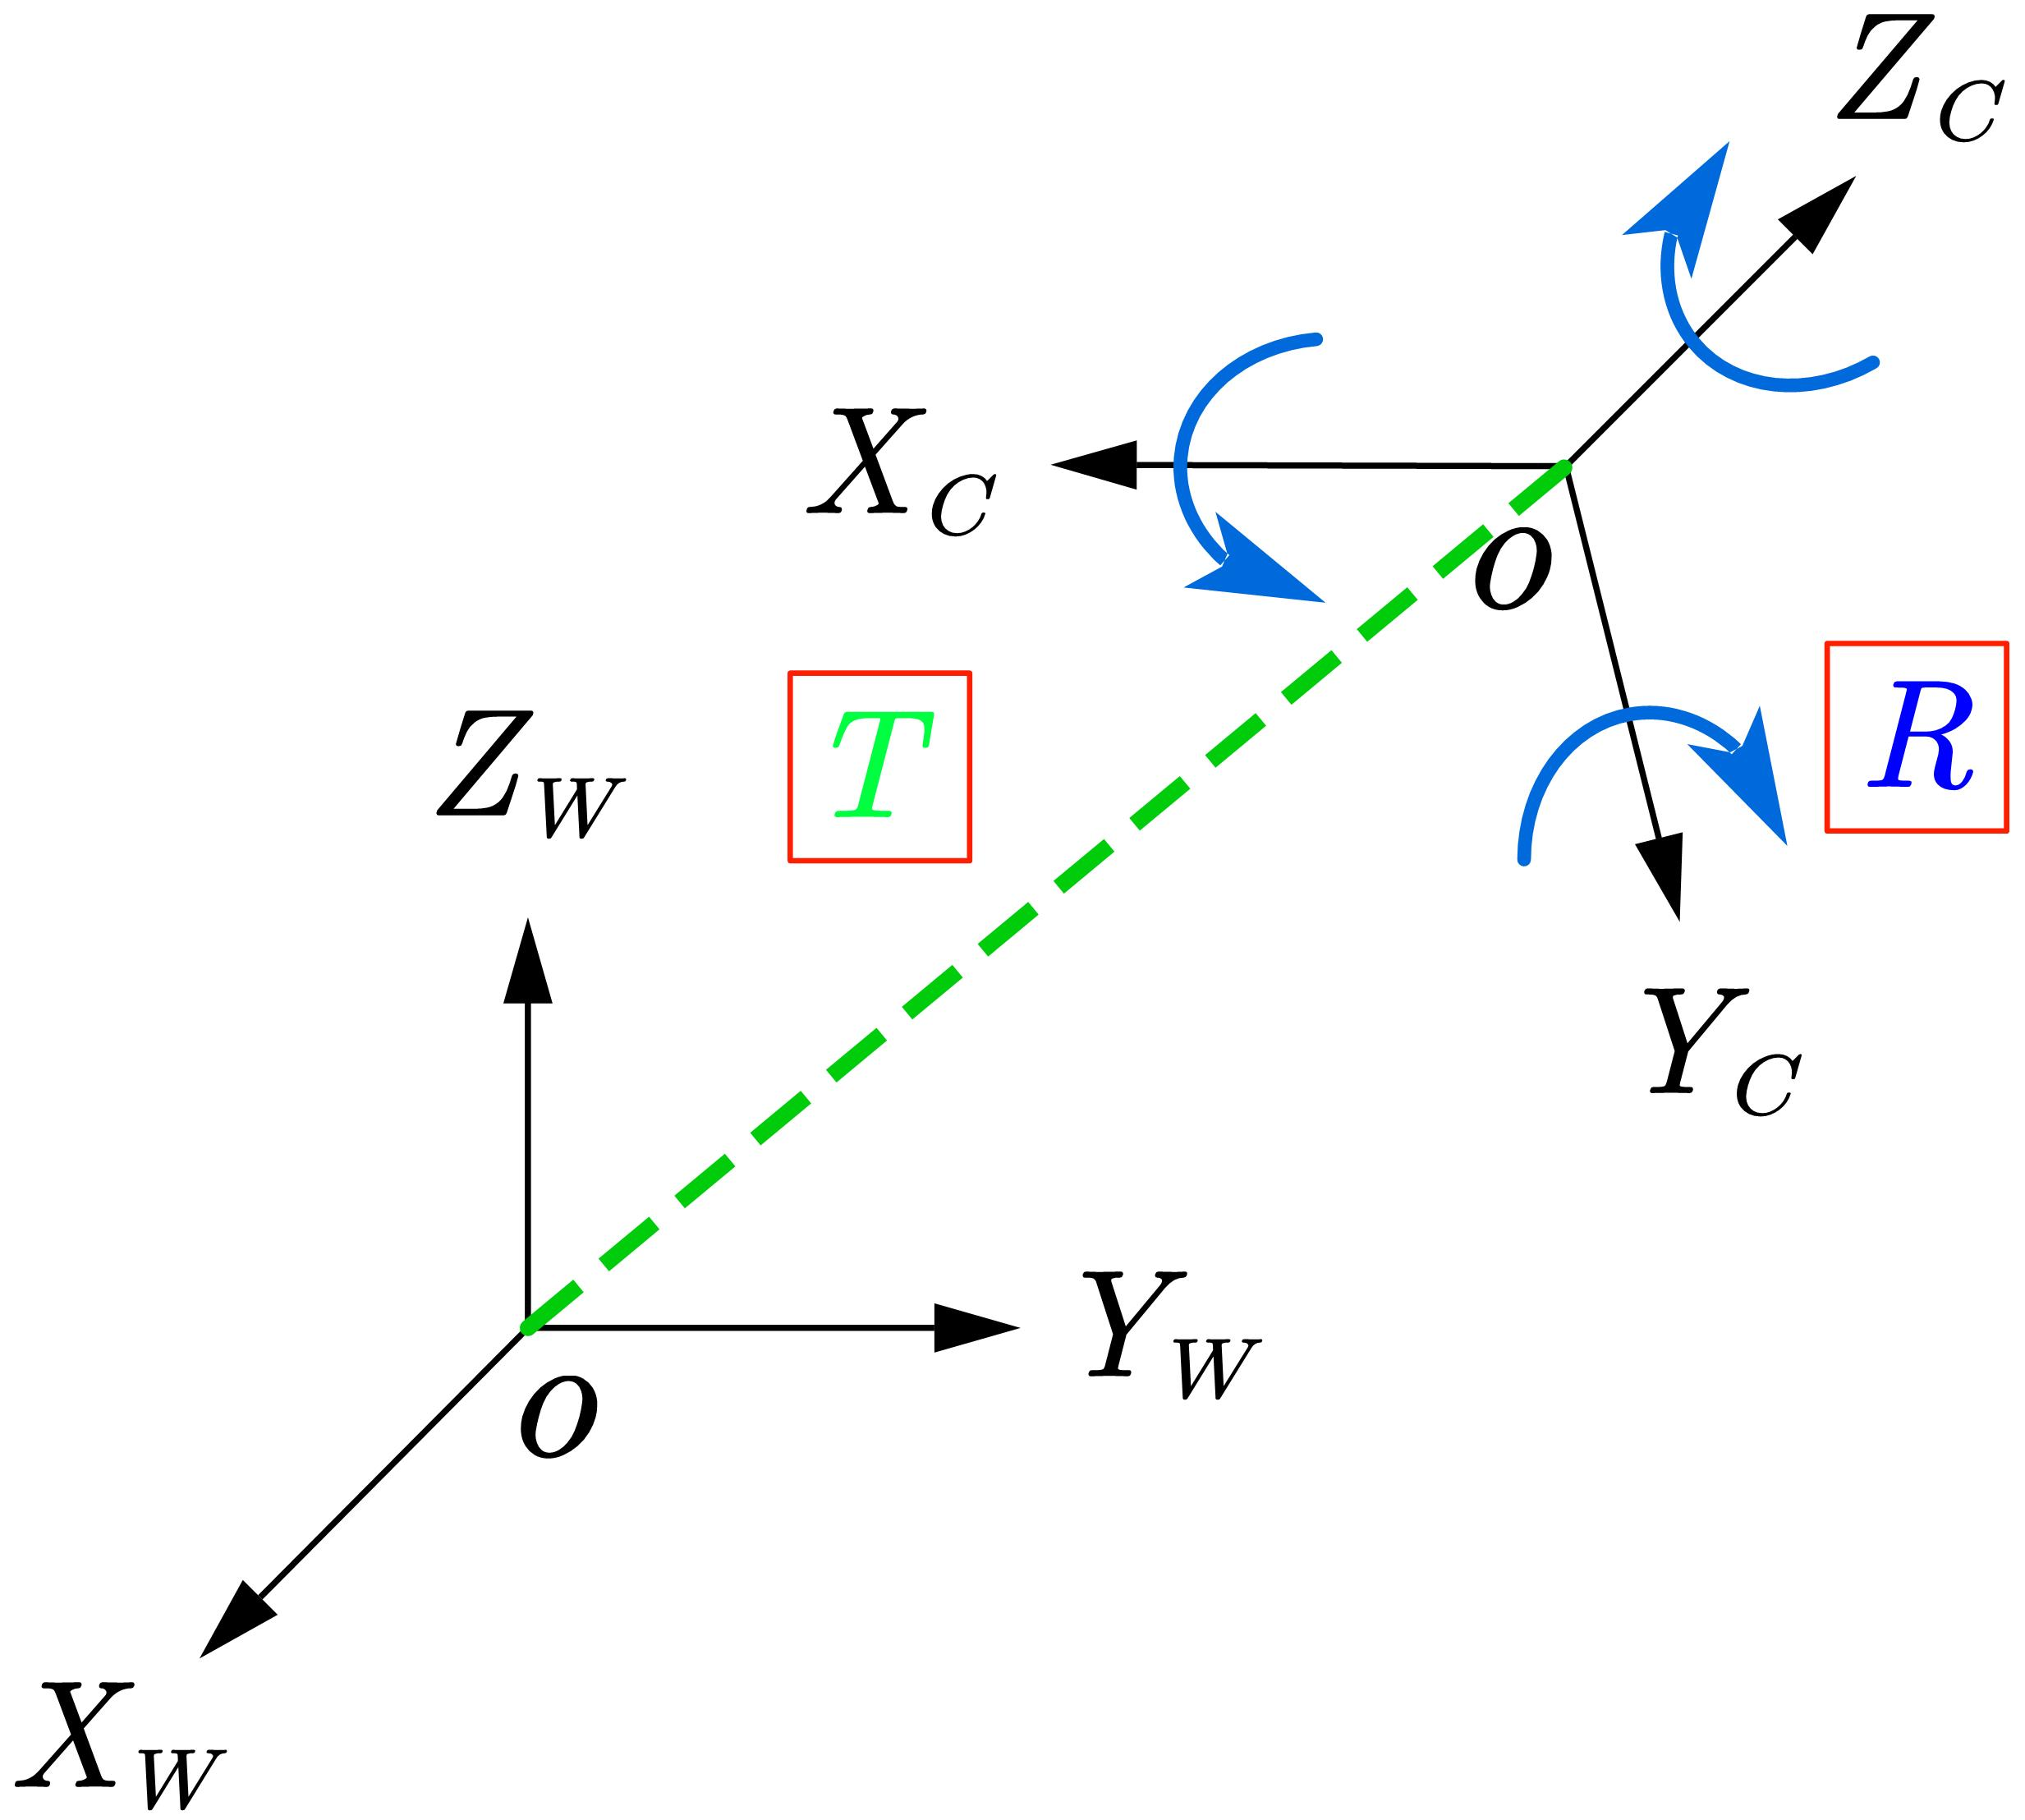
\includegraphics[scale=0.8]{世界坐标系到相机坐标系}
				\caption{世界坐标系到相机坐标系}
				\label{世界坐标系到相机坐标系-图}
			\end{center}
		\end{figure}
		其数学描述如式\ref{世界坐标系到相机坐标系-公式}所示:
		\begin{gather}
			\left[ \begin{array}{c}
				X_C\\
				Y_C\\
				Z_C\\
				1\\
			\end{array} \right] =\left[ \begin{matrix}
				R&		T\\
				0&		1\\
			\end{matrix} \right] \left[ \begin{array}{c}
				X_W\\
				Y_W\\
				Z_W\\
				1\\
			\end{array} \right] \label{世界坐标系到相机坐标系-公式}
		\end{gather}	

		\item \textbf{相机坐标系$\Longrightarrow$图像坐标系}
		
		根据小孔成像模型,我们有如图\ref{三角形相似-图}所示的相似关系,其数学描述如式(\ref{三角形相似-式1}),(\ref{三角形相似-式2})所示:
		\begin{figure}[H]
			\begin{center}
				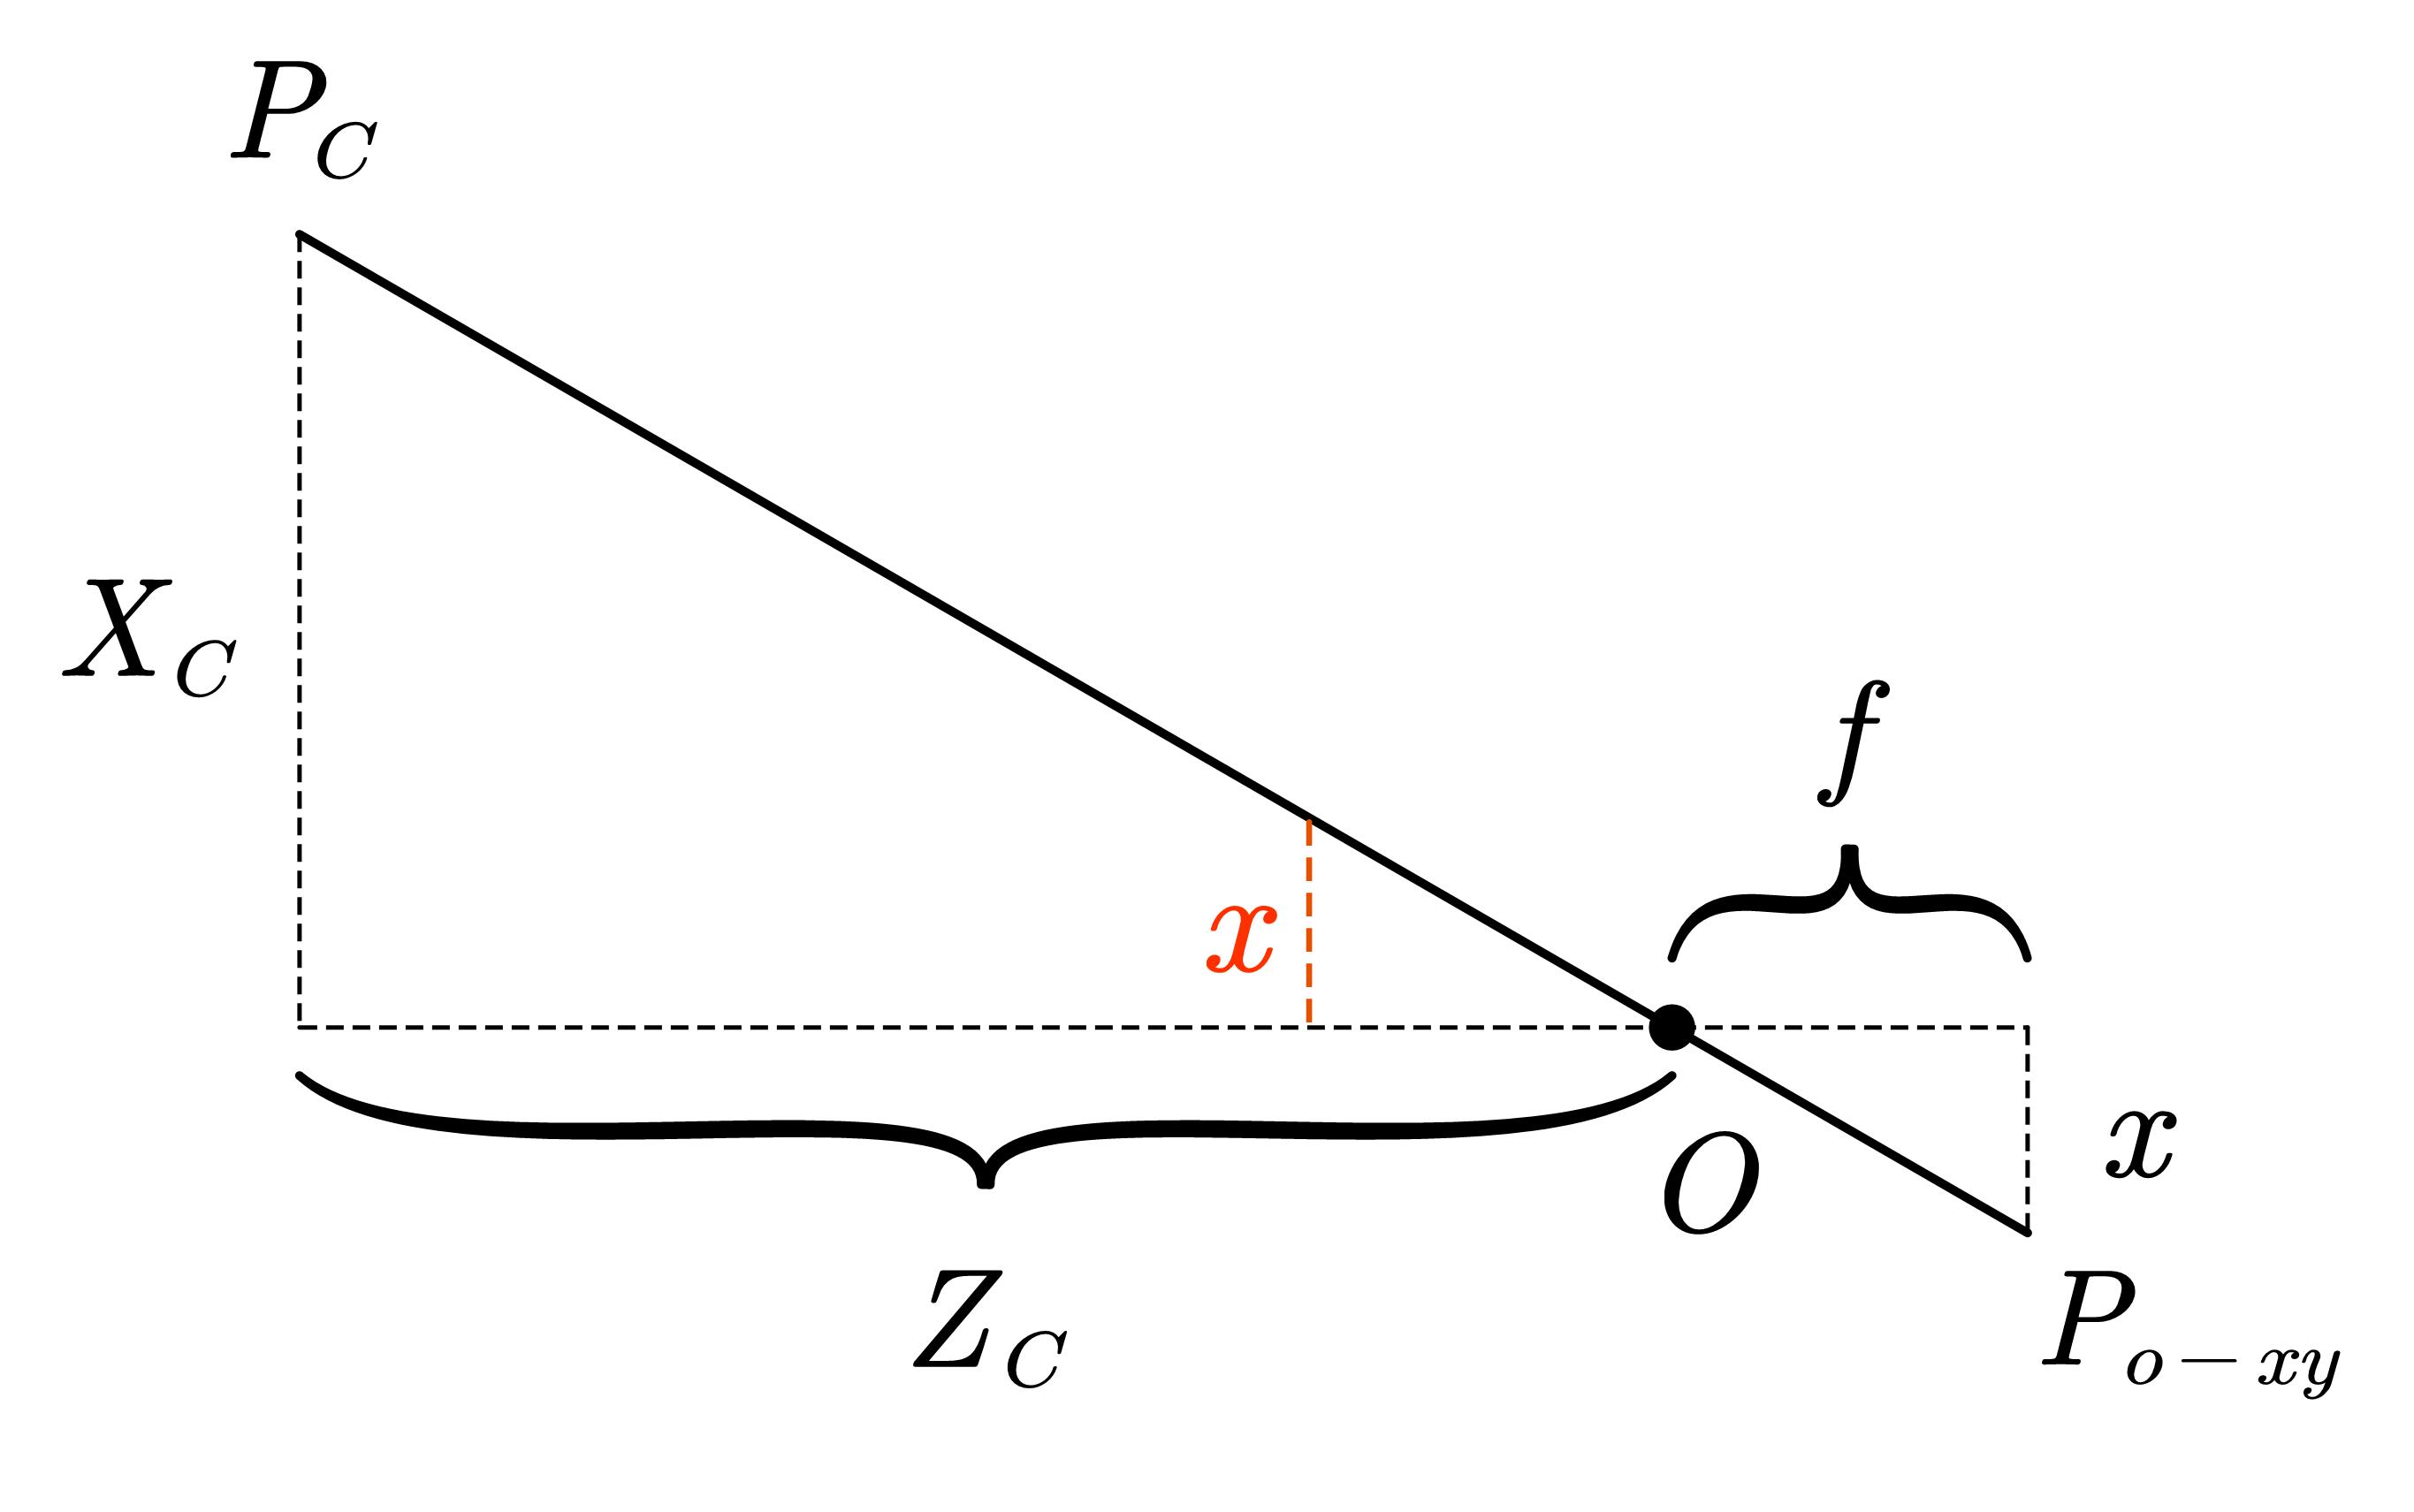
\includegraphics[scale=0.65]{小孔成像模型}
				\caption{三角形相似}
				\label{三角形相似-图}
			\end{center}
		\end{figure}
		\begin{gather}
			{\small \left[ \begin{array}{c}
					x\\
					y\\
					1\\
				\end{array} \right] =\left[ \begin{matrix}
					f/Z_C&		0&		0&		0\\
					0&		f/Z_C&		0&		0\\
					0&		0&		1/Z_C&		0\\
				\end{matrix} \right] \left[ \begin{array}{c}
					X_C\\
					Y_C\\
					Z_C\\
					1\\
				\end{array} \right]   }	\label{三角形相似-式1}
		\end{gather}
		\begin{gather}
			{\small Z_C\cdot \left[ \begin{array}{c}
					x\\
					y\\
					1\\
				\end{array} \right] =\left[ \begin{matrix}
					f&		0&		0&		0\\
					0&		f&		0&		0\\
					0&		0&		1&		0\\
				\end{matrix} \right] \left[ \begin{array}{c}
					X_C\\
					Y_C\\
					Z_C\\
					1\\
				\end{array} \right]  } \label{三角形相似-式2}
		\end{gather}	
		\item \textbf{图像坐标系$\Longrightarrow$像素坐标系}
		
		如图\ref{相机坐标系到像素坐标系-图}所示,图像坐标系和像素坐标系并不完全重合,像素坐标系的原点在一张图像的左上角。
		\begin{figure}[H]
			\begin{center}
				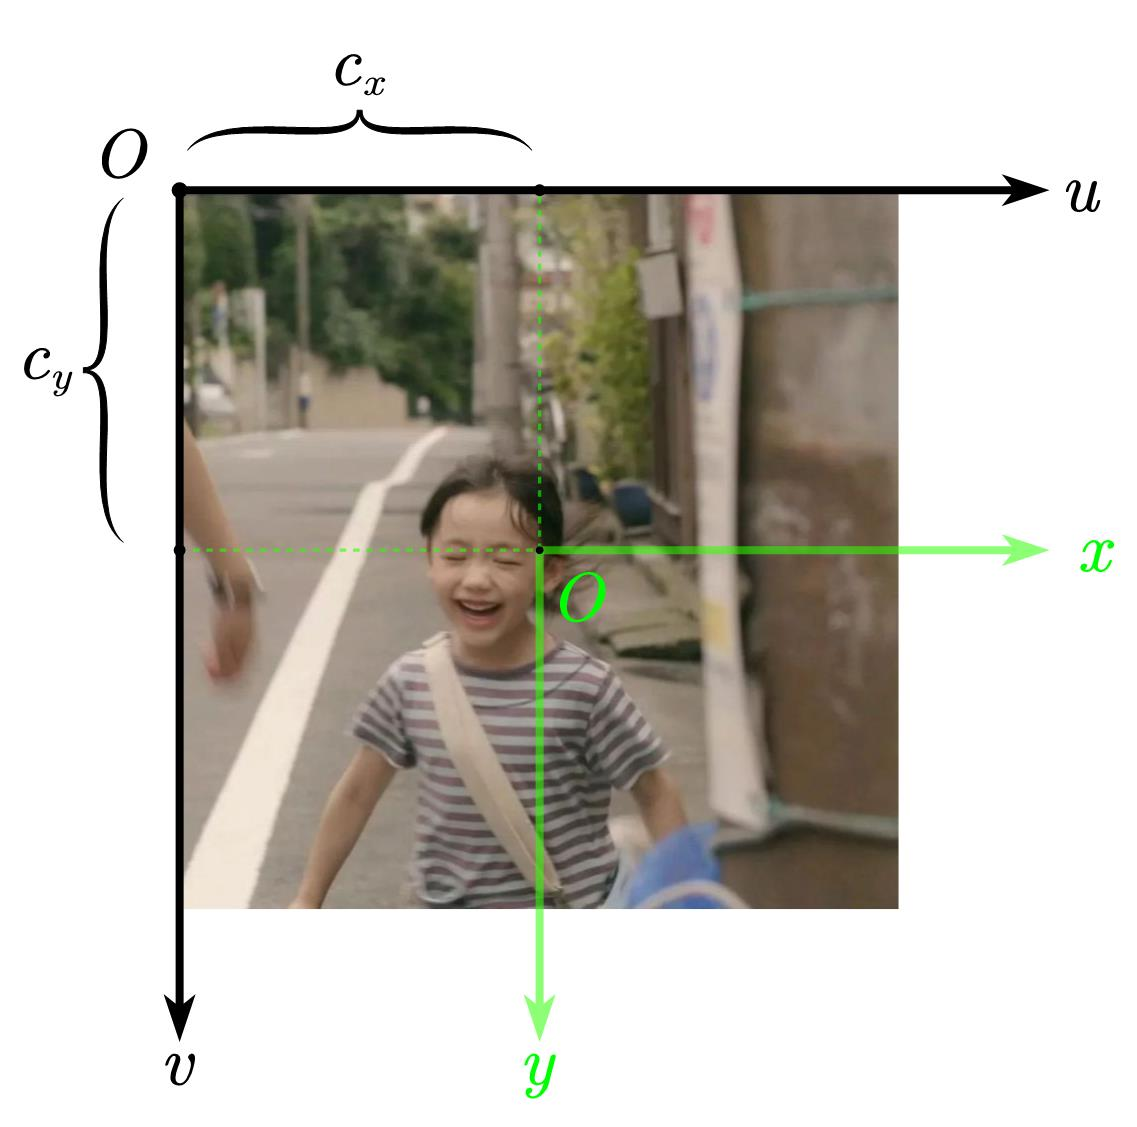
\includegraphics[scale=0.35]{相机坐标系到像素坐标系}
				\caption{相机坐标系到像素坐标系}
				\label{相机坐标系到像素坐标系-图}
			\end{center}
		\end{figure}
其数学描述如式(\ref{相机坐标系到像素坐标系-式})所示:
	\begin{equation}\label{相机坐标系到像素坐标系-式}
	\begin{aligned}
		{\small \left[ \begin{array}{c}
				u\\
				v\\
				1\\
			\end{array} \right] =\left[ \begin{matrix}
				1/d_x&		0&		c_x\\
				0&		1/d_y&		c_y\\
				0&		0&		1\\
			\end{matrix} \right] \left[ \begin{array}{c}
				x\\
				y\\
				1\\
			\end{array} \right]  }  	
	\end{aligned}	
\end{equation}

其中各参数含义如下:
\begin{itemize}
	\item $d_x,d_y$:像元尺寸
	\item $f_x,f_y$:各轴归一化焦距
		$$\begin{cases}
		f_x={{f}\big/{d_x}}\\
		f_y={{f}\big/{d_y}}\\
	\end{cases}$$
	\item $c_x$,$c_y$:两坐标系偏移量
\end{itemize}
\end{itemize}

我们将以上三种变换统一起来,就得到了世界坐标系到像素坐标系之间的对应关系,其推导如下所示:
\begin{tcolorbox}[colback=JungleGreen!10!Cerulean!15,colframe=CornflowerBlue!60!Black]
	
		\begin{equation*}
	\begin{aligned}
		\left[ \begin{array}{c}
			u\\
			v\\
			1\\
		\end{array} \right] &=\left[ \begin{matrix}
			1/d_x&		0&		c_x\\
			0&		1/d_y&		c_y\\
			0&		0&		1\\
		\end{matrix} \right] \left[ \begin{array}{c}
			x\\
			y\\
			1\\
		\end{array} \right] 
		\\
		&=\left[ \begin{matrix}
			1/d_x&		0&		c_x\\
			0&		1/d_y&		c_y\\
			0&		0&		1\\
		\end{matrix} \right] \left[ \begin{matrix}
			f/Z_C&		0&		0&		0\\
			0&		f/Z_C&		0&		0\\
			0&		0&		1/Z_C&		0\\
		\end{matrix} \right] \left[ \begin{array}{c}
			X_C\\
			Y_C\\
			Z_C\\
			1\\
		\end{array} \right] 
		\\
		&=\left[ \begin{matrix}
			1/d_x&		0&		c_x\\
			0&		1/d_y&		c_y\\
			0&		0&		1\\
		\end{matrix} \right] \left[ \begin{matrix}
			f/Z_C&		0&		0&		0\\
			0&		f/Z_C&		0&		0\\
			0&		0&		1/Z_C&		0\\
		\end{matrix} \right] \left[ \begin{matrix}
			R&		T\\
			0&		1\\
		\end{matrix} \right] \left[ \begin{array}{c}
			X_W\\
			Y_W\\
			Z_W\\
			1\\
		\end{array} \right] 
		\\
		&=\frac{1}{Z_C}\cdot \left[ \begin{matrix}
			1/d_x&		0&		c_x\\
			0&		1/d_y&		c_y\\
			0&		0&		1\\
		\end{matrix} \right] \cdot \left[ \begin{matrix}
			f&		0&		0&		0\\
			0&		f&		0&		0\\
			0&		0&		1&		0\\
		\end{matrix} \right] \cdot \left[ \begin{matrix}
			R&		T\\
		\end{matrix} \right] \cdot \left[ \begin{array}{c}
			X_W\\
			Y_W\\
			Z_W\\
			1\\
		\end{array} \right] 
	\end{aligned}
\end{equation*}	
\end{tcolorbox}
不妨令式(\ref{内参矩阵求解-内参矩阵})称为内参矩阵:
	\begin{align}
	M_1&={\color{blue} \left[ \begin{matrix}
			1/d_x&		0&		c_x\\
			0&		1/d_y&		c_y\\
			0&		0&		1\\
		\end{matrix} \right] \cdot \left[ \begin{matrix}
			f&		0&		0&		0\\
			0&		f&		0&		0\\
			0&		0&		1&		0\\
		\end{matrix} \right] } \nonumber
	\\
	&=\left[ \begin{matrix}
		f_x&		0&		c_x\\
		0&		f_y&		c_y\\
		0&		0&		1\\
	\end{matrix} \right] \label{内参矩阵求解-内参矩阵}
\end{align}


不妨令式(\ref{外参矩阵})称为外参矩阵:
	\begin{gather}
	M_2={\color{blue} \left[ \begin{matrix}
			R&		T\\
		\end{matrix} \right] } \label{外参矩阵}
\end{gather}

不妨假设以下:
\begin{itemize}
		\item 棋盘格角点的$Z_W=0$
		\item 令$s ={{1}\big/{Z_C}}$,称为缩放因子
		\item 令$R=\left[ \begin{matrix}
	r_1&		r_2&		r_3\\
\end{matrix} \right] $
\end{itemize}

代入以上假设条件,我们重新整理该等式,式(\ref{单应矩阵包含内外参矩阵})中$H$矩阵称为单应性矩阵,包含了相机的内、外参矩阵和缩放因子,反映世界坐标系与像素坐标系之间的对应关系。
	\begin{align}
	\left[ \begin{array}{c}
		u\\
		v\\
		1\\
	\end{array} \right] &=\frac{1}{{\color{blue} Z_C}}\cdot M_1\cdot \left[ \begin{matrix}
		{\color{blue} r_1}&		{\color{blue} r_2}&		{\color{blue} r_3}&		T\\
	\end{matrix} \right] \cdot \left[ \begin{array}{c}
		X_W\\
		Y_W\\
		{\color{blue} Z_W}\\
		1\\
	\end{array} \right] \nonumber
	\\
	&=s \cdot M_1\cdot \left[ \begin{matrix}
		r_1&		r_2&		{\color[RGB]{255, 0, 128} r_3}&		T\\
	\end{matrix} \right] \cdot \left[ \begin{array}{c}
		X_W\\
		Y_W\\
		{\color[RGB]{255, 0, 128} Z_W}\\
		1\\
	\end{array} \right] \nonumber
	\\
	&=s \cdot M_1\cdot \left[ \begin{matrix}
		r_1&		r_2&		T\\
	\end{matrix} \right] \cdot \left[ \begin{array}{c}
		X_W\\
		Y_W\\
		1\\
	\end{array} \right] \nonumber
	\\
	&=\boldsymbol{H}\cdot \left[ \begin{array}{c}
		X_W\\
		Y_W\\
		1\\
	\end{array} \right]  	\label{单应矩阵包含内外参矩阵}	
\end{align}

单应性 (Homography)是射影几何中的概念,又称为射影变换、透视变换,如图\ref{单应性1}所示,反映两个平面之间的映射关系

\begin{figure}[H]
	\begin{center}
		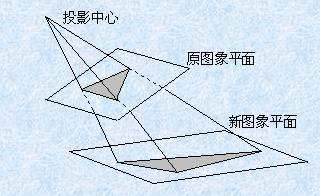
\includegraphics[scale=0.7]{射影变换}
		\caption{单应性1}
		\label{单应性1}
	\end{center}
\end{figure}

单应性在不同的应用场景有不同的理解,对图\ref{单应性2}中现实世界的同一点,在不同视角图像上的同一点可以用式(\ref{单应性对应-公式})对应起来
\begin{gather}\label{单应性对应-公式}
	p_2=H\cdot p_1
\end{gather}
\begin{figure}[H]
	\begin{center}
		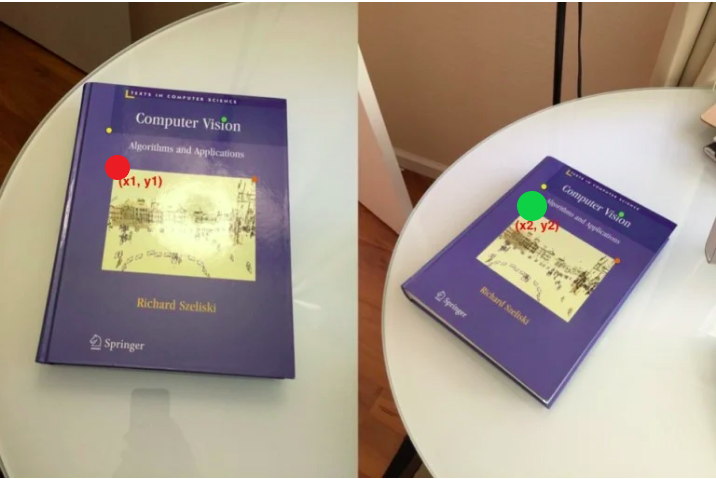
\includegraphics[scale=0.3]{单应性}
		\caption{单应性2}
		\label{单应性2}
	\end{center}
\end{figure}

上述推导的基础都是基于齐次坐标 (Homogeneous Coordinate)这一概念,在欧式空间 (笛卡尔空间)中,同一平面的平行直线不相交,但在透视空间却可以相交,如图\ref{平行线相交}所示的铁轨在无穷原点交于一点
\begin{figure}
\begin{center}
	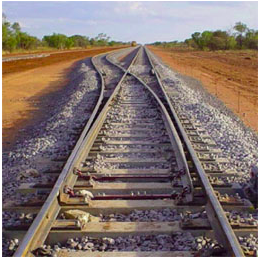
\includegraphics[scale=0.5]{平行线相交}
	\caption{两条铁轨在无穷远点看似相交}
	\label{平行线相交}
\end{center}
\end{figure}

于是为了统一欧式空间与透视空间中同一平面平行直线可以相交这一问题,引入齐次坐标来表示无穷远点,可以认为在欧式空间中同一平面平行直线可以在无穷远点处相交。


\begin{tcolorbox}[title=\textbf{使用 N+1 维坐标来代替 N 维坐标},colback=SeaGreen!10!CornflowerBlue!10,colframe=RoyalPurple!55!Aquamarine!100!]
\begin{equation*}
	\begin{aligned}
		\mathop {\left( x,y,w \right) \Longleftrightarrow \left( \frac{x}{w},\frac{y}{w} \right)} \limits_{\mathrm{Homogeneous}    \quad        \mathrm{Cartesian}}			
	\end{aligned}
\end{equation*}
\end{tcolorbox}



\begin{tcolorbox}[title=\textbf{为什么叫齐次性?\footnote{表示二维平面的无穷远点$\left( x,y,0 \right) \Longleftrightarrow \left( \infty ,\infty \right) $}},colback=SeaGreen!10!CornflowerBlue!10,colframe=RoyalPurple!55!Aquamarine!100!]
	\begin{equation*}
		\begin{aligned}
			&	\left( 1,2,3 \right) \Rightarrow \left( \frac{1}{3},\frac{2}{3} \right) 
			\\
			&	\left( 2,4,6 \right) \Rightarrow \left( \frac{2}{6},\frac{4}{6} \right) =\left( \frac{1}{3},\frac{2}{3} \right) 
			\\
			&	\left( {\color[RGB]{0, 0, 240} a,2a,3a} \right) \Rightarrow \left( \frac{a}{3a},\frac{2a}{3a} \right) =\left( \frac{1}{3},\frac{2}{3} \right) 
		\end{aligned}	
	\end{equation*}
\end{tcolorbox}

几何变换,主要包括平移、旋转、缩放,用矩阵来表达这些变换时,平移是矩阵相加,旋转和缩放则是矩阵相乘,$p' = m_1*p+ m_2$,综合起来表示为$p' = M*p$,所以,引入齐次坐标可以{\color[RGB]{128, 0, 255} \text{合并矩阵运算中的乘法和加法}}。




\subsubsection{经典标定方法:张正友标定法}

张正友标定法是张正友教授于1998年提出的二维平面棋盘格的相机标定方法。传统标定法的标定板是三维的,需要非常精确,不仅难以制作,实验起来也非常困难,而张正友标定法克服了传统标定法需要的高精度标定物的缺点,只需打印出来的黑白棋盘格就可以,同时提高了精度,便于操作。

首先构造目标点与图像点之间的单应性矩阵,即世界坐标与像素坐标之间的映射关系。然后利用正交约束条件分离出相机内参与外参的初始值。最后使用极大似然估计优化结果,得到左右相机的内外参矩阵。

\begin{itemize}
	\item 求解单应矩阵
	\begin{tcolorbox}
		[colback = Emerald!10, colframe = cyan!40!black, title = (1)化为齐次坐标]
		令$p_1=\left( x_1,y_1 \right) ^T,p_2=\left( x_2,y_2 \right) ^T,H=\left[ \begin{matrix}
			h_{11}&		h_{12}&		h_{13}\\
			h_{21}&		h_{22}&		h_{23}\\
			h_{31}&		h_{32}&		h_{33}\\
		\end{matrix} \right] =\left[ \begin{matrix}
			h_1&		h_2&		h_3\\
		\end{matrix} \right]  $,$H$把$p_1$映射到$p_2$,对应齐次坐标为:$p_1=\left( x_1,y_1,1 \right) ^T,p_2=\left( x_2,y_2,1 \right) ^T$
	\end{tcolorbox}
	
	\begin{tcolorbox}
		[colback = Emerald!10, colframe = cyan!40!black, title = (2)单应性矩阵的自由度]
		在等式(\ref{单应性对应-公式})两端同时乘以常数$a$原等式化为$a\cdot p_2={\color{blue} a\cdot H}\cdot p_1$,新得到的单应性矩阵$aH$和原单应性矩阵$H$的作用相同,因为齐次坐标乘以常数后保持不变,所以虽然$H$有九个元素,但自由度却为8,我们常令$h_{33}=1$以简化计算。
	\end{tcolorbox}
	
	\begin{tcolorbox}
		[colback = Emerald!10, colframe = cyan!40!black, title = (3)求解单应矩阵]
					\begin{align}
			\left[ \begin{array}{c}
				x_2\\
				y_2\\
				1\\
			\end{array} \right] &=\left[ \begin{matrix}
				h_{11}&		h_{12}&		h_{13}\\
				h_{21}&		h_{22}&		h_{23}\\
				h_{31}&		h_{32}&		h_{33}\\
			\end{matrix} \right] \cdot \left[ \begin{array}{c}
				x_1\\
				y_1\\
				1\\
			\end{array} \right] \nonumber
			\\
			& \Rightarrow \begin{cases}
				x_2=h_{11}\cdot x_1+h_{12}\cdot y_1+h_{13}\\
				y_2=h_{21}\cdot x_1+h_{22}\cdot y_1+h_{23}\\
				1=h_{31}\cdot x_1+h_{32}\cdot y_1+h_{33}\\
			\end{cases}\Rightarrow \begin{cases}
				x_2=\frac{h_{11}\cdot x_1+h_{12}\cdot y_1+h_{13}}{h_{31}\cdot x_1+h_{32}\cdot y_1+h_{33}}\\
				y_2=\frac{h_{21}\cdot x_1+h_{22}\cdot y_1+h_{23}}{h_{31}\cdot x_1+h_{32}\cdot y_1+h_{33}}\\
			\end{cases} \nonumber
			\\
			& \Rightarrow \begin{cases}
				x_2\left( h_{31}\cdot x_1+h_{32}\cdot y_1+h_{33} \right) -\left( h_{11}\cdot x_1+h_{12}\cdot y_1+h_{13} \right) =0\\
				y_2\left( h_{31}\cdot x_1+h_{32}\cdot y_1+h_{33} \right) -\left( h_{21}\cdot x_1+h_{22}\cdot y_1+h_{23} \right) =0\\
			\end{cases} \nonumber
			\\
			& \Rightarrow \begin{cases}
				-h_{11}\cdot x_1-h_{12}\cdot y_1-h_{13}+h_{31}\cdot x_1x_2+h_{32}\cdot y_1+h_{33}=0\\
				-h_{21}\cdot x_1-h_{22}\cdot y_1-h_{23}+h_{31}\cdot x_1y_2+h_{32}\cdot y_1+h_{33}=0\\
			\end{cases}  \nonumber \\
			& \Rightarrow A\cdot h=\boldsymbol{0} \label{线性解法}
		\end{align}	
		\begin{itemize}
			\item $A=\left[ \begin{matrix}
				x_1&		y_1&		1&		0&		0&		0&		x_1x_2&		y_1&		1\\
				0&		0&		0&		x_1&		y_1&		1&		x_1y_2&		y_1&		1\\
			\end{matrix} \right] $
			\item $h=\left[ \begin{matrix}
				h_{11}&		h_{12}&		h_{13}&		h_{21}&		h_{22}&		h_{23}&		h_{31}&		h_{32}&		{\color[RGB]{0, 0, 240} h_{33}}\\
			\end{matrix} \right] ^T$
			\vspace{0.8em}
			\item 棋盘格一个脚点对应两个方程,对应$A$矩阵的两行,所以只需四个脚点就可以将$A$垒到八行,$A\cdot h=\boldsymbol{0}$就存在唯一解。
		\end{itemize}
	\end{tcolorbox}
	
	\begin{tcolorbox}
		[colback = Emerald!10, colframe = cyan!40!black, title = (4)理想与现实]
		\begin{itemize}
			\item 以上只是理论的推导,在真实的场景中,我们计算的点中都会包含噪声。比如点的位置偏差几个像素,甚至出现特征点对误匹配的现象,如果仅用四个点对来计算单应矩阵,那么会出现很大的误差。
			\item  因此为了计算的更加准确,一般采用远大于4个点来计算单应矩阵,假如有$n$对,就能将$A$矩阵垒到$2n$行。
			\item 如果方程\ref{线性解法}采用线性解法很难得到最优解,所以一般采取其它的优化方法如SVD奇异值分解、Levenberg-Marquarat(LM)算法\footnote{一种结合了梯度下降法和高斯-牛顿法的迭代法,用于求解非线性最小二乘问题}等进行求解。
		\end{itemize}
	\end{tcolorbox}

	\item 求解内参矩阵
	
	单应矩阵包括内参和外参矩阵,而内参矩阵更方便求解,之后再求外参矩阵,求解思路是利用旋转向量的约束关系,根据式(\ref{单应矩阵包含内外参矩阵}),我们可以得到以下关系:\\
	\begin{align}
		H &=\left[ \begin{matrix}
			h_1&		h_2&		h_3\\
		\end{matrix} \right] \nonumber
		\\
		&=s \cdot M_1\cdot M_2 \nonumber
		\\
		&=s \cdot M_1\cdot \left[ \begin{matrix}
			r_1&		r_2&		T\\
		\end{matrix} \right] \nonumber
		\\
		&	\Rightarrow \begin{cases}
			h_1=sM_1r_1\\
			h_2=sM_1r_2\\
			h_3=sM_1T\\
		\end{cases} \nonumber
		\\
		&	\Rightarrow \begin{cases}
			r_1=s ^{-1} {M_1}^{-1}h_1\\
			r_2=s ^{-1} {M_1}^{-1}h_2\\
			T=s ^{-1} {M_1}^{-1}h_3\\
		\end{cases}
	\end{align}

根据旋转向量的约束条件:
\begin{formal}
\begin{description}
	\item[约束条件1:旋转向量正交] 
	\begin{align}
		& {r_1}^Tr_2=0 \nonumber
		\\
		& \Rightarrow {h_1}^T{\color{blue} \left( s ^{-1} {M_1}^{-1} \right) ^Ts ^{-1} {M{\color{blue} _1}}^{-1}}h_2=0 \label{内参矩阵的求解约束条件1}
	\end{align}
	\item[约束条件2:旋转向量长度相等(旋转不改变尺度)] 
	\begin{align}
		& \left\| r_1 \right\| =\left\| r_2 \right\| =1 \nonumber
		\\
		& \Rightarrow {r_1}^Tr_1={r_2}^Tr_2 \nonumber
		\\
		& \Rightarrow {h_1}^T{\color{blue} \left( s ^{-1}{M_1}^{-1} \right) ^Ts ^{-1}{M{\color{blue} _1}}^{-1}}h_1={h_2}^T{\color{blue} \left( s ^{-1}{M_1}^{-1} \right) ^Ts ^{-1}{M{\color{blue} _1}}^{-1}}h_2 \label{内参矩阵的求解约束条件2}
	\end{align}
\end{description}
\end{formal}

令$M_1=\left[ \begin{matrix}
	f_x&		{\color{blue} \gamma \footnote{畸变因子,非常小,一般忽略} }&		c_x\\
	0&		f_y&		c_y\\
	0&		0&		1\\
\end{matrix} \right] $,再令$B={\color{blue} \left( s ^{-1}{M_1}^{-1} \right) ^Ts ^{-1}{M{\color{blue} _1}}^{-1}}$,我们得到:\\
\begin{align}
	B&=\left( s^{-1}{M_1}^{-1} \right) ^Ts^{-1}{M_1}^{-1}={\color{blue} \lambda }\left( {M_1}^{-1} \right) ^T{M_1}^{-1} \label{内参矩阵的求解-B矩阵}
	\\
	&=\lambda \cdot\left[ \begin{matrix}
		\frac{1}{{f_x}^2}&		-\frac{\gamma}{{f_x}^2f_y}&		\frac{c_y\gamma -c_xf_y}{{f_x}^2f_y}\\
		-\frac{\gamma}{{f_x}^2f_y}&		\frac{\gamma ^2}{{f_x}^2{f_y}^2}+\frac{1}{{f_y}^2}&		-\gamma \frac{c_y\gamma -c_xf_y}{{f_x}^2{f_y}^2}-\frac{c_y}{{f_y}^2}\\
		\frac{c_y\gamma -c_xf_y}{{f_x}^2f_y}&		-\gamma \frac{c_y\gamma -c_xf_y}{{f_x}^2{f_y}^2}-\frac{c_y}{{f_y}^2}&		\frac{\left( c_y\gamma -c_xf_y \right) ^2}{{f_x}^2{f_y}^2}+\frac{{c_y}^2}{{f_y}^2}+1\\
	\end{matrix} \right] \nonumber
	\\
	&	=\left[ \begin{matrix}
		b_{11}&		b_{12}&		b_{13}\\
		b_{21}&		b_{22}&		b_{23}\\
		b_{31}&		b_{32}&		b_{33}\\
	\end{matrix} \right] \nonumber
\end{align}\\
$B$为对称阵,真正有用的元素只有6个,根据约束条件(\ref{内参矩阵的求解约束条件1})(\ref{内参矩阵的求解约束条件2})及式(\ref{内参矩阵的求解-B矩阵}),我们得到:\\
\begin{align}
	\begin{cases}
		{h_1}^TBh_2=0\\
		{h_1}^TBh_1={h_2}^TBh_2\\
	\end{cases}\Leftrightarrow {h_i}^TBh_j \label{内参矩阵的求解-H矩阵的化简}
\end{align}

令$H=\left[ \begin{matrix}
h_1&		h_2&		h_3\\
\end{matrix} \right] $的第$i$列列向量:$h_i=\left[ \begin{matrix}
h_{1i}&		h_{2i}&		h_{3i}\\
\end{matrix} \right] ^T$,将$h_i$代入式(\ref{内参矩阵的求解-H矩阵的化简})进一步化简得:
		\begin{align}
	{h_i}^TBh_j&=\left[ \begin{matrix}
		h_{1i}&		h_{2i}&		h_{3i}\\
	\end{matrix} \right] _{1\times 3}\cdot \left[ \begin{matrix}
		{\color{blue} b_{11}}&		b_{12}&		b_{13}\\
		{\color{blue} b_{21}}&		{\color{blue} b_{22}}&		b_{23}\\
		{\color{blue} b_{31}}&		{\color{blue} b_{32}}&		{\color{blue} b_{33}}\\
	\end{matrix} \right] _{3\times 3}\cdot \left[ \begin{array}{c}
		h_{1j}\\
		h_{2j}\\
		h_{3j}\\
	\end{array} \right] _{3\times 1} \nonumber
	\\
	&	={\left[ \begin{array}{c}
			h_{1i}\cdot b_{11}+h_{2i}\cdot b_{21}+h_{3i}\cdot b_{31}\\
			h_{1i}\cdot b_{12}+h_{2i}\cdot b_{22}+h_{3i}\cdot b_{32}\\
			h_{1i}\cdot b_{13}+h_{2i}\cdot b_{23}+h_{3i}\cdot b_{33}\\
		\end{array} \right] _{{\color[RGB]{240, 0, 0} 1}\times 3}}^T\cdot \left[ \begin{array}{c}
		h_{1j}\\
		h_{2j}\\
		h_{3j}\\
	\end{array} \right] _{3\times {\color[RGB]{240, 0, 0} 1}} \nonumber
	\\
	&	=\left[ \begin{array}{c}
		h_{1i}h_{1j}\\
		h_{1j}h_{2i}+h_{2j}h_{1i}\\
		h_{2i}h_{2j}\\
		h_{1j}h_{3i}+h_{3j}h_{1i}\\
		h_{3i}h_{3j}\\
		h_{2j}h_{3i}+h_{3j}h_{2i}\\
	\end{array} \right] ^T\left[ \begin{array}{c}
		b_{11}\\
		b_{12}\\
		b_{22}\\
		b_{13}\\
		b_{33}\\
		b_{23}\\
	\end{array} \right] \label{内参矩阵的求解-hb-vb代换}
\end{align}

在式(\ref{内参矩阵的求解-hb-vb代换})中,令:
\begin{align}
	v_{ij}&=\left[ \begin{array}{c}
		h_{1i}h_{1j}\\
		h_{1j}h_{2i}+h_{2j}h_{1i}\\
		h_{2i}h_{2j}\\
		h_{1j}h_{3i}+h_{3j}h_{1i}\\
		h_{3i}h_{3j}\\
		h_{2j}h_{3i}+h_{3j}h_{2i}\\
	\end{array} \right] ^T
	\\
	b&=\left[ \begin{array}{c}
		b_{11}\\
		b_{12}\\
		b_{22}\\
		b_{13}\\
		b_{33}\\
		b_{23}\\
	\end{array} \right] \label{内参矩阵求解-b}
\end{align}

		根据式(\ref{内参矩阵的求解-H矩阵的化简}),得到:\\
\begin{align}
	\begin{cases}\label{内参矩阵求解-每张图片都可以得到两个等式}
		{v_{12}}^Tb=0\\
		\left( {v_{11}}^T-{v_{22}}^T \right) b\\
	\end{cases}
\end{align}
由于每张图像都可以得到一个单应矩阵,将每个矩阵构建成如式(\ref{内参矩阵求解-每张图片将矩阵垒两行})进一步整理得到:
\begin{align}\label{内参矩阵求解-每张图片将矩阵垒两行}
	\left[ \begin{array}{c}
		{v_{12}}^T\\
		{v_{11}}^T-{v_{22}}^T\\
	\end{array} \right] \cdot b=0
\end{align}


可以用之前求解的单应矩阵$H$来得到$v_{11},v_{12},v_{22}$,并且每张图片都可以得到如如式(\ref{内参矩阵求解-每张图片都可以得到两个等式})的两个等式,可以将式(\ref{内参矩阵求解-每张图片将矩阵垒两行})中的矩阵垒两行,而如式(\ref{内参矩阵求解-b})所示,$b$只含有6个未知数,因此至少保证图片数大于等于3张才能解出$b$。


根据式(\ref{内参矩阵求解-每张图片将矩阵垒两行})求出的$b$,我们就可以得到$B$,而根据式(\ref{内参矩阵的求解-B矩阵}),我们有:\\
\begin{align}
	\begin{cases}
		f_x=\sqrt{{{\lambda}\big/{b_{11}}}}\\ \nonumber
		f_y=\sqrt{{{\lambda b_{11}}\big/{\left( b_{11}b_{22}-{b_{12}}^2 \right)}}}\\ \nonumber
		c_x={{\gamma  c_y}\big/{f_y}}-{{b_{13}f_x}\big/{\lambda}}\\ \nonumber
		c_y={{\left( b_{12}b_{13}-b_{11}b_{23} \nonumber \right)}\big/{\left( b_{11}b_{22}-{b_{12}}^2 \right)}}\\
		\gamma =-{{b_{12}{f_x}^2f_y}\big/{\lambda}}\\ \nonumber
		\lambda =b_{33}-{{\left[ {b_{13}}^2+c_y\left( b_{12}b_{13}-b_{11}b_{23} \right) \right]}\big/{b_{11}}} \nonumber
	\end{cases}
\end{align}
%	\begin{shaded}
	代入式(\ref{内参矩阵求解-内参矩阵}),我们就求出了内参矩阵$M_1=\left[ \begin{matrix}
		f_x&		\gamma&		c_x\\
		0&		f_y&		c_y\\
		0&		0&		1\\
	\end{matrix} \right] $

	\item 求解外参矩阵
	
此时根据求得的内参矩阵$M_1$和单应矩阵$H$,可以根据下面两个约束条件继续求得外参矩阵$M_2$:

\begin{formal}
\begin{description}
	\item[旋转向量互相垂直] 
	\begin{align}
		\begin{cases}
			r_1=s^{-1}{M_1}^{-1}h_1\\ \nonumber
			r_2=s^{-1}{M_1}^{-1}h_2\\ \nonumber
			r_3=r_1\times r_2\\ \nonumber
			T=s^{-1}{M_1}^{-1}h_3 \nonumber
		\end{cases}
	\end{align}
	\item[旋转向量长度为1]
	\begin{align}
		\left\| r_1 \right\| =\left\| s^{-1}{M_1}^{-1}h_1 \right\| =1 \nonumber
	\end{align}
\end{description}
\end{formal}
\end{itemize}




\subsubsection{单目相机标定求解左右相机内外参矩阵}
\begin{itemize}
	\item 制作黑白棋盘格标定板
	\item 不同角度采集图像
	\item 特征点(角点)检测
	\begin{itemize}
		\item 灰度化
		\item 滤波
		\item 二值化
		\item Canndy边缘检测
		\item 棋盘格轮廓定位
		\item 提取角点初始坐标
		\item 角点坐标的亚像素化处理
	\end{itemize}
	\item 基于张正友标定法求解左右相机内外参
	\item 求解畸变参数
	\item Levenberg-Marquard(LM)算法对畸变参数进行优化
	
以上实验均不考虑相机镜头带来的畸变影响,但在实际中相机镜头却有一定的畸变(主要为径向畸变),于是为了提高标定精度,我们采用Levenberg-Marquart (LM)算法对标定结果进行优化。L-M 非线性最小二乘算法综合并改进了Gauss-Newton 算法和梯度下降算法。该算法在迭代过程中,可对参数进行自适应调整,从而快速收敛到最优解。
\end{itemize}
\subsubsection{双目相机标定求解左右相机位姿关系}
\begin{itemize}
	\item 平行式双目视觉系统
	\item 汇聚式双目视觉系统
	\item 极线约束简化特征点匹配
	\item 双目标定求解左右相机位姿关系
\end{itemize}
\subsubsection{机器人手眼标定实现物品抓取}

在相机标定实验中,我们得到了三维世界坐标系的物体相对于相机坐标系的位置关系,采用机械手臂进行物体抓取时,相机通常在机械手臂末端执行器的位置,为了得到三维世界坐标系的物体相对于机械手臂基座的位置关系,从而通过机械人逆运动学求解D-H矩阵,控制各关节的旋转角度到达指定位置实现抓取操作,我们需要进行手眼标定。

如图\ref{手眼标定分类}所示,根据相机安装位置的不同,我们将手眼标定分为以下两种:
\begin{itemize}
	\item Eye-in-hand(眼在手上)
	
	相机安装在机械臂末端执行器位置,标定板不动,随着机械臂的移动,实现了相机从不同角度拍摄图像
	\item Eye-to-hand(眼在手外)
	
	相机固定不动,标定板固定在机械臂末端执行器位置,让标定板出现在相机视野中,随着机械臂的移动,实现了相机从不同角度拍摄图像
	\begin{figure}[H]
		\centering  %居中
		\subfigure[Eye-in-hand]{   %第一张子图
			\begin{minipage}{7cm}
				\centering    %子图居中
				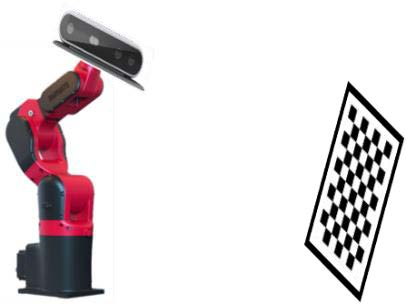
\includegraphics[scale=0.8]{Eye-in-hand}  %以pic.jpg的0.5倍大小输出
			\end{minipage}
		}
		\subfigure[Eye-to-hand]{ %第二张子图
			\begin{minipage}{7cm}
				\centering    %子图居中
				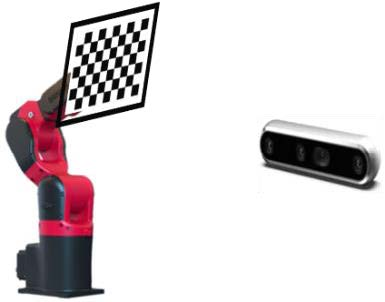
\includegraphics[scale=0.8]{Eye-to-hand}
			\end{minipage}
		}
		\caption{手眼标定示意图}    %大图名称
		\label{手眼标定分类}    %图片引用标记
	\end{figure}
\end{itemize}


\subsection{实施方案}
\begin{itemize}
	\item 查阅资料了解机器视觉的概念,熟练掌握相应的数理基础:矩阵与坐标系的变换,学习数字图像处理,对双目摄像头采集到的图像进行简单的预处理以提取物体特征,掌握张正友标定方法,利用MATLAB的Stereo Calibration工具箱对预处理的图像进行相机标定,得到三维世界的物体相对于相机的位置关系,掌握手眼标定的知识,利用MATLAB标定的结果对物体进行手眼标定,得到三维世界相对于机械臂基座的相对位置关系,从而控制机械臂完成定位抓取
	\item 打印黑白棋盘格标定板,搭建双目摄像机实验平台,安装MATLAB Stereo Calibration工具箱,GitHub下载双目摄像机图像显示软件,完成软硬件准备工作
	\item 双目相机拍照获取图像,对图像进行预处理排除噪声,之后将其导入MATLAB进行相机标定,得到左右相机的内外参矩阵及其相对位置关系,之后进行机器人手眼标定,最后利用得到的结果控制机械臂完成对物体的定位抓取。
	\item 以上工作不考虑相机镜头的畸变,因此在考虑相机镜头畸变的情况下,我们用LM算法对畸变参数进行优化
	
\end{itemize}










\section{参考文献}








\section{进度安排(按周说明)}
\begin{enumerate}
	\item 第一周-第三周:了解机器视觉的概念,学会相应的数理基础知识,了解相机标定的工作原理,掌握张正友标定法,学会数字图像处理的基本知识,学习c++基本语法并搭建其编程环境。
	\item 第四周-第六周:准备相应的软硬件,配置视觉标定环境,完成迎检工作内容。
	\item 第七周-第十周:进行标定有关的实验,实现设计要求的功能。
	\item 第十一周-第十三周:翻译外文资料,按要求编写设计说明书
	\item 第十四周-第十五周:毕业设计收尾工作,准备答辩。
	
\end{enumerate}
\section{指导教师审批意见}
\begin{flushright}
	指导教师:\quad \quad(签名)\\
	年\quad 月 \quad 日
\end{flushright}

\end{document}